\chapter[RESULTADOS]{\textbf {RESULTADOS}}

O software construído por este projeto, o \emph{Open Gait Analytics} versão 0.1, foi interamente construído pelo autor desta obra, e está liberado no site \url{https://github.com/rob-nn/open_gait_analytics}, sob a licença \emph{MIT}. Para saber mais sobre esta licença veja \ref{mit_sec}.
A intenção do autor é aumentar as chances de que futuras versões do software sejam construídas, não importando se serão comerciais ou gratuitas.
Importante frizar também que o software continuará sendo desenvolvido pelo autor nos próximos meses.

O software em si é composto por dois módulos que são apresentados na Figura \ref{tela1}. O principal objetivo neste momento é atrair pesquisadores da área de análise de marcha para o software. Por isso há o módulo simulação, no qual o pesquisador poderá simular sinais.
O módulo de análise visa atender tanto a pesquisadores, quanto a profissionais da área clínica. Neste momento o software é mais um protótipo funcional do que algo pronto para o mercado, portanto o uso por profissionais da área clínica não é recomendado ainda.

\begin{figure}[ht]
	\centering
	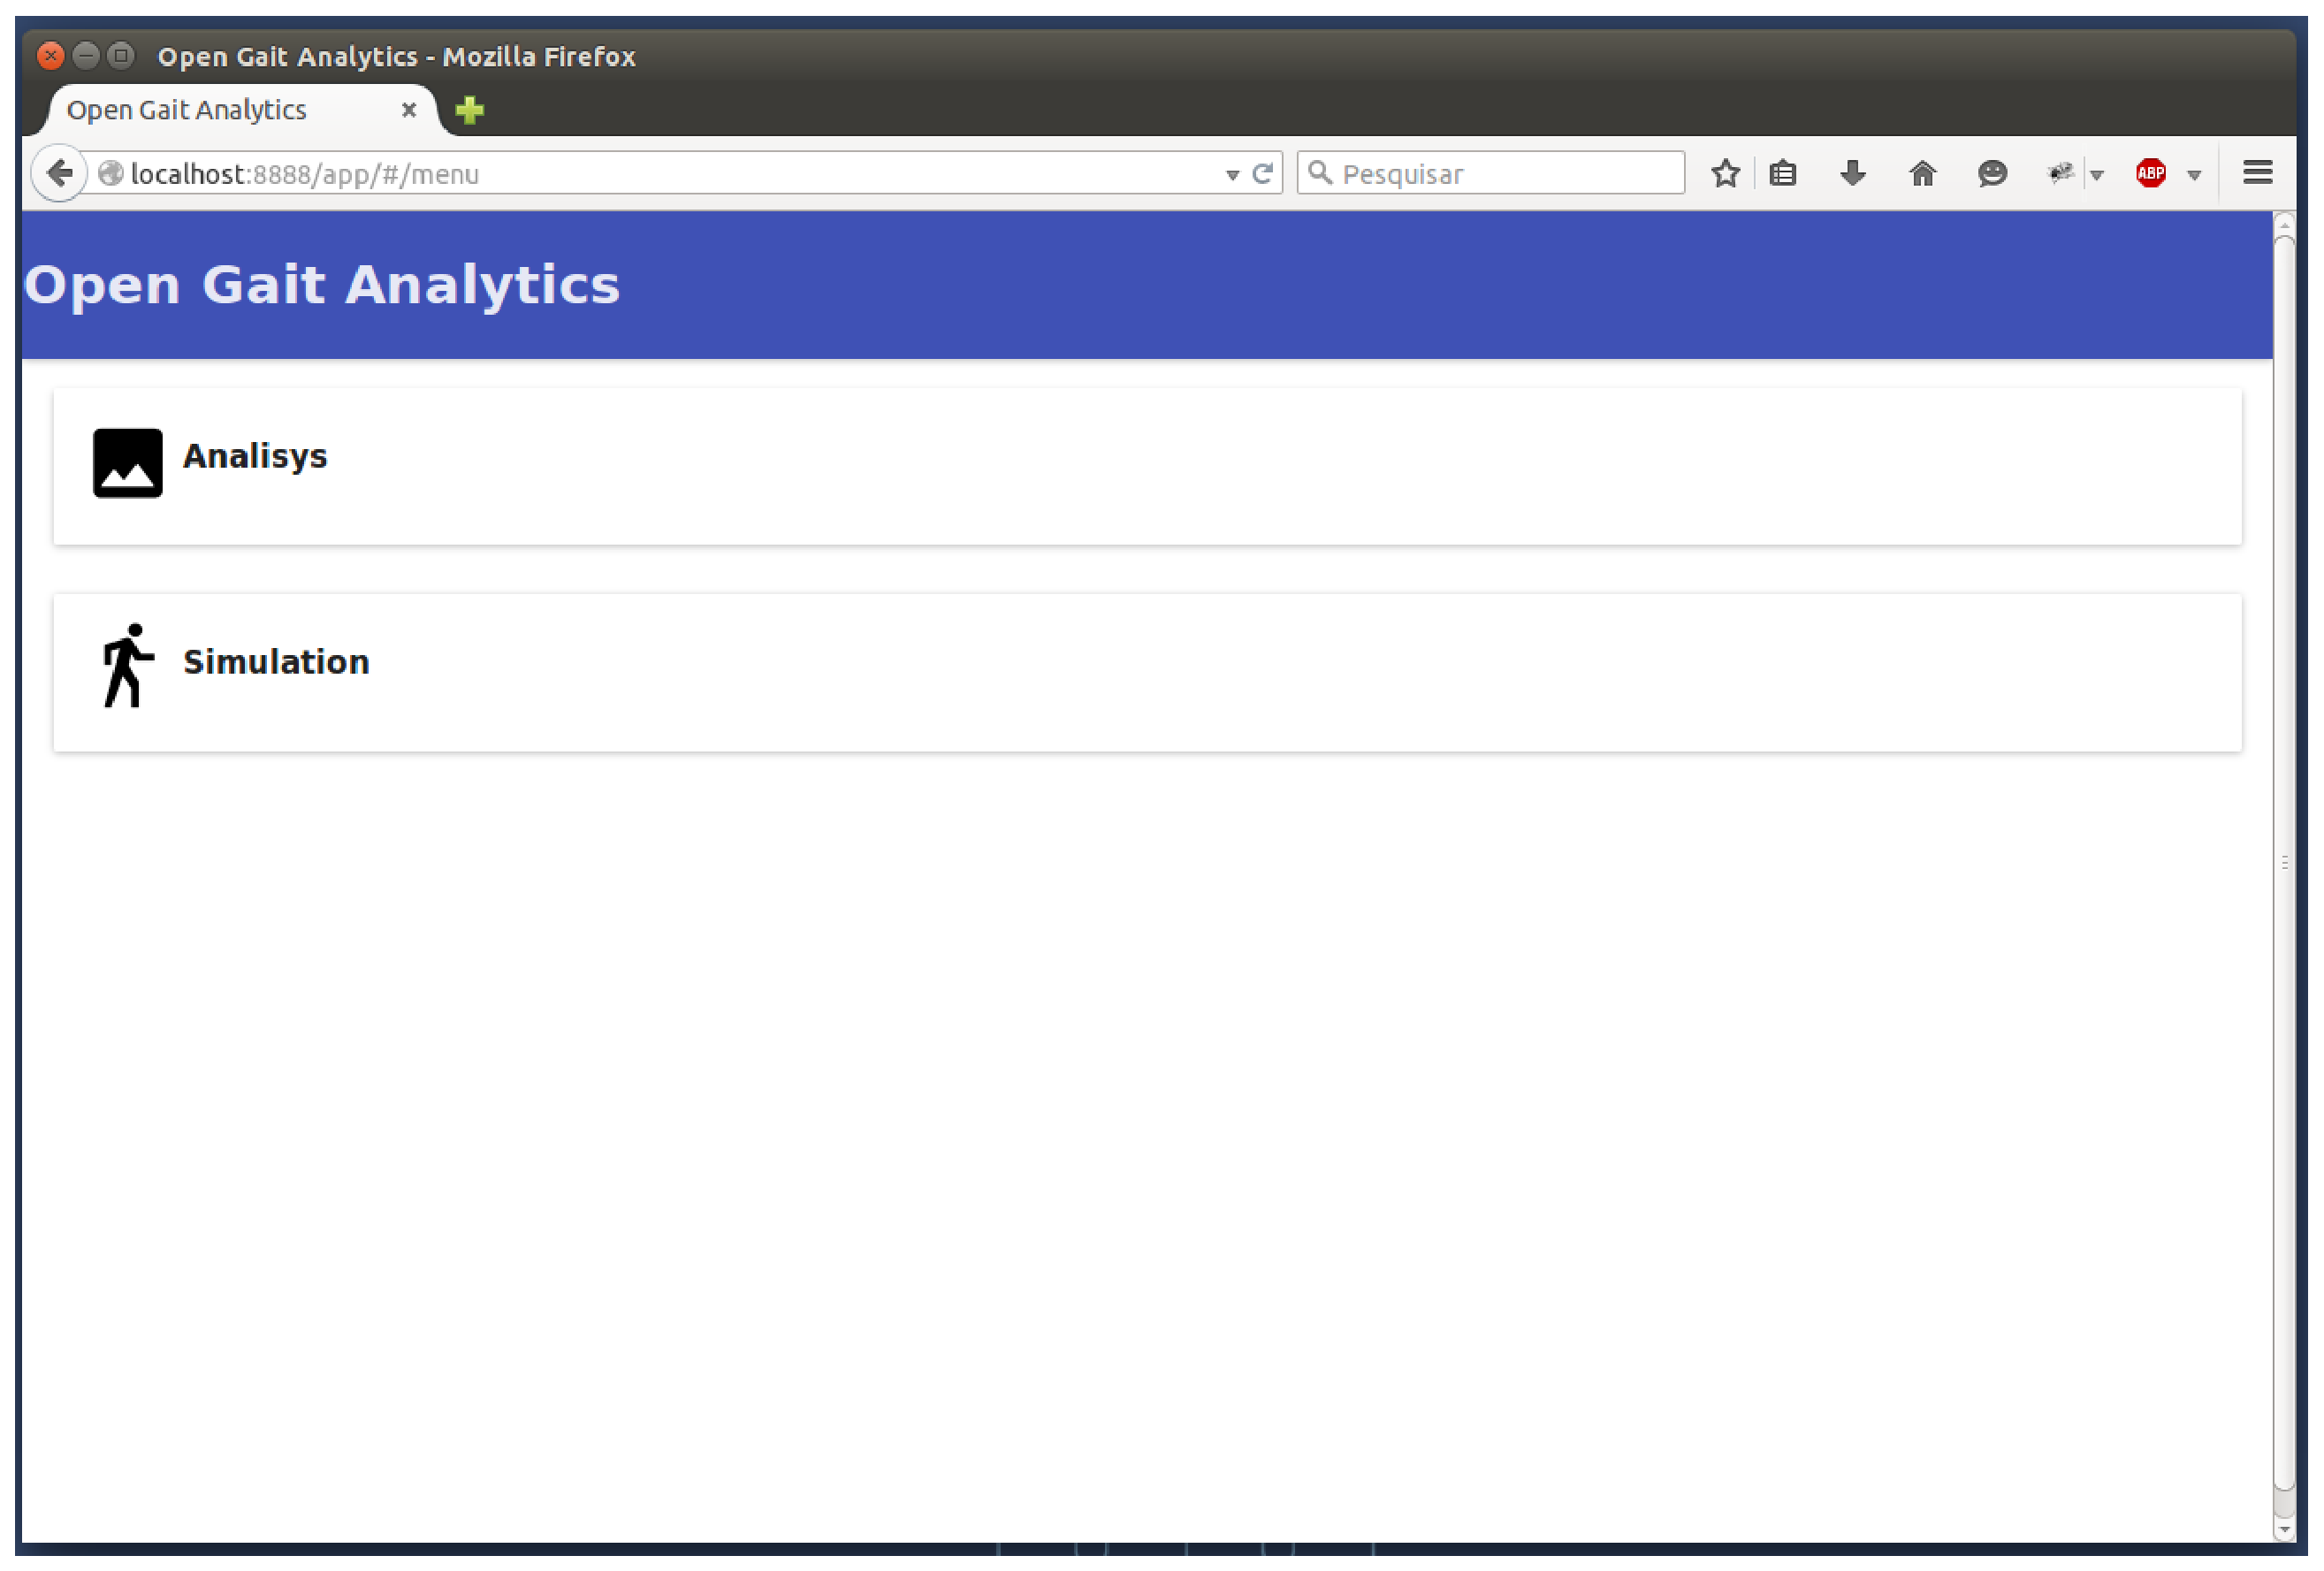
\includegraphics[width=15cm]{figuras/tela1.eps}
	\caption{Tela de seleção dos módulos.}
	\label{tela1}
\end{figure}

\section{Módulo de Análise}
Neste fase o software conta apenas com análise de movimentos, com sinais oriundos de marcadores passivos de superfície, captados por câmeras, usando o software \emph{QTM}. 
No \emph{QTM} é feita a conversão dos dados para o formato \emph{Matlab} que é reconheciodo pelo sistema construído.

A primeira tela deste módulo pode ser vista na Figura \ref{tela2}. Este tela apresenta a listagem de pacientes, cadastrados no sistema. O botão abaixo a direita, é a função para adicionar novos pacientes.

\begin{figure}[ht]
	\centering
	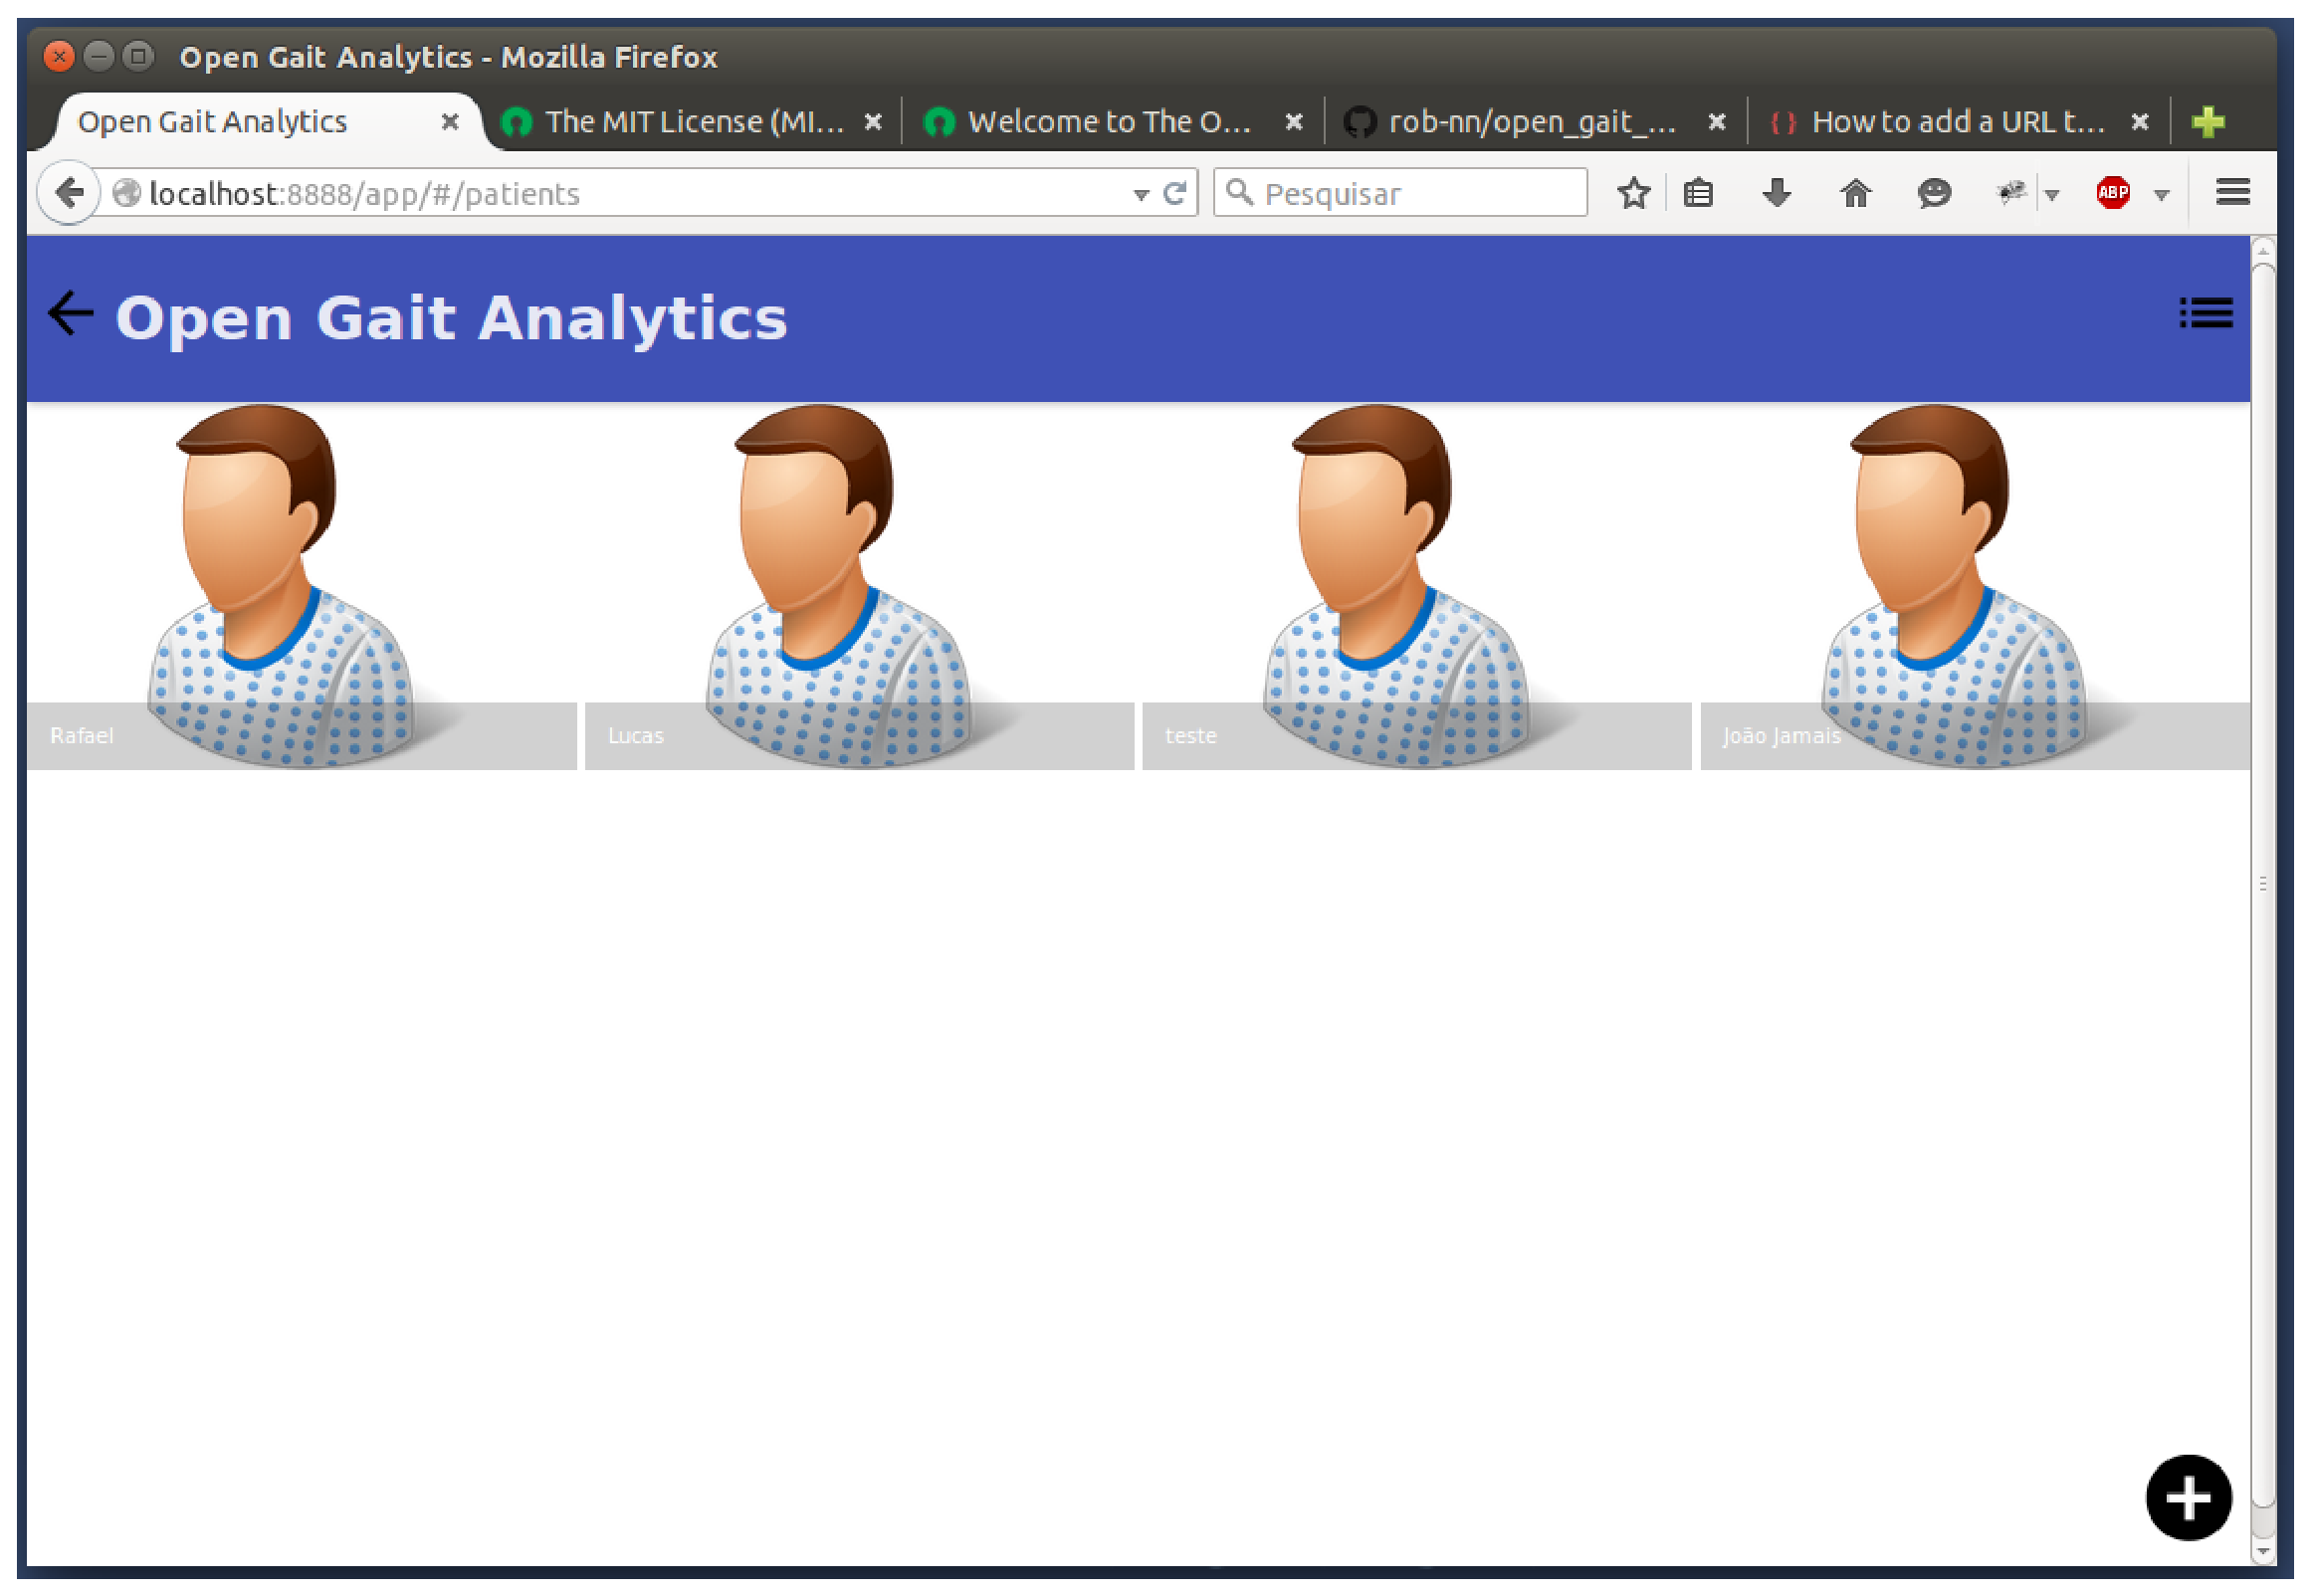
\includegraphics[width=15cm]{figuras/tela2.eps}
	\caption{Tela com a listagem de pacientes.}
	\label{tela2}
\end{figure}

A Figura \ref{tela3} mostra as informações do paciente que devem ser preenchidas ao se executar a função adicionar paciente. Esta tela é uma adaptação da ficha de avaliação que está na obra \citeonline{VeraReg}.

\begin{figure}[ht]
	\centering
	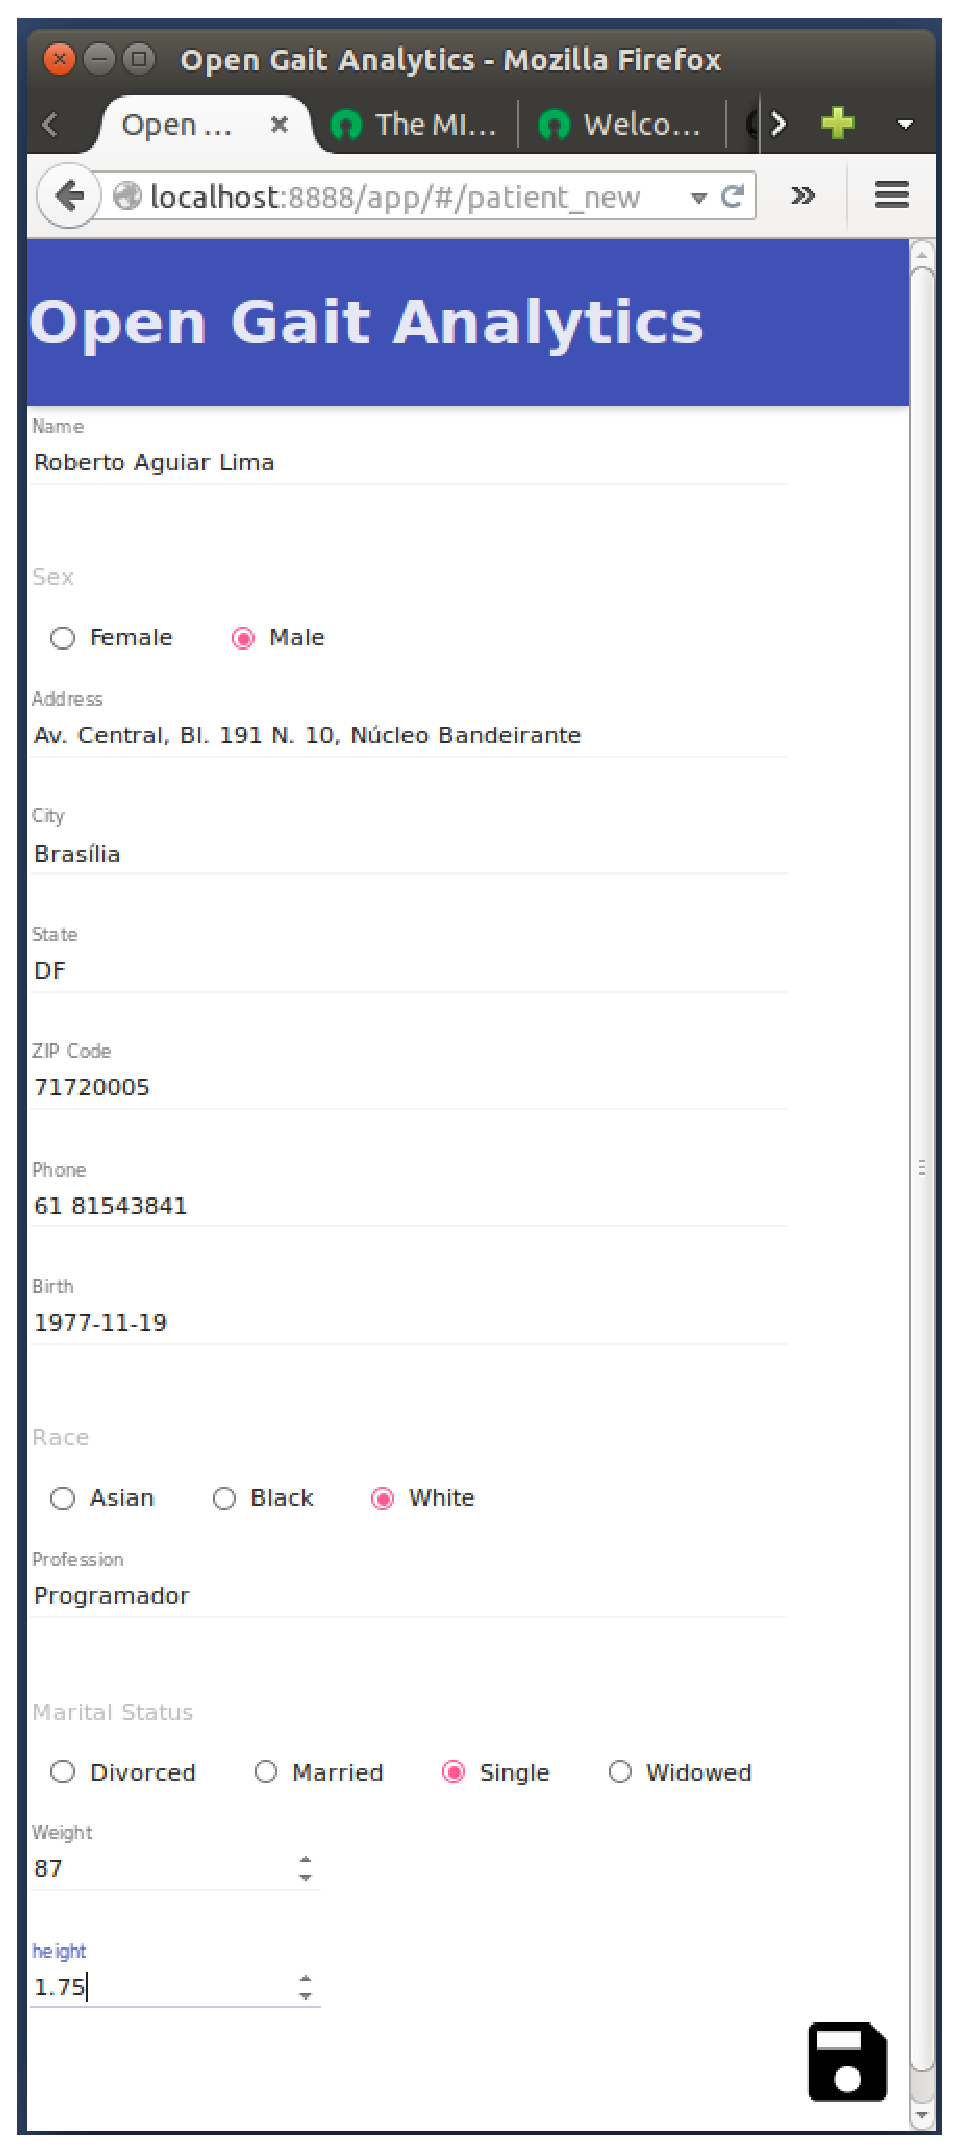
\includegraphics[width=7cm]{figuras/tela3.eps}
	\caption{Informações do paciente.}
	\label{tela3}
\end{figure}

Ao se selecionar um paciente da tela mostrada na Figura \ref{figura2}, a tela da Figura \ref{tela4} aparece. No caso em questão, nenhuma coleta de dados foi carregada para o paciente. Logo o próximo passo é adicionar uma nova amostra de marcha.

\begin{figure}[ht]
	\centering
	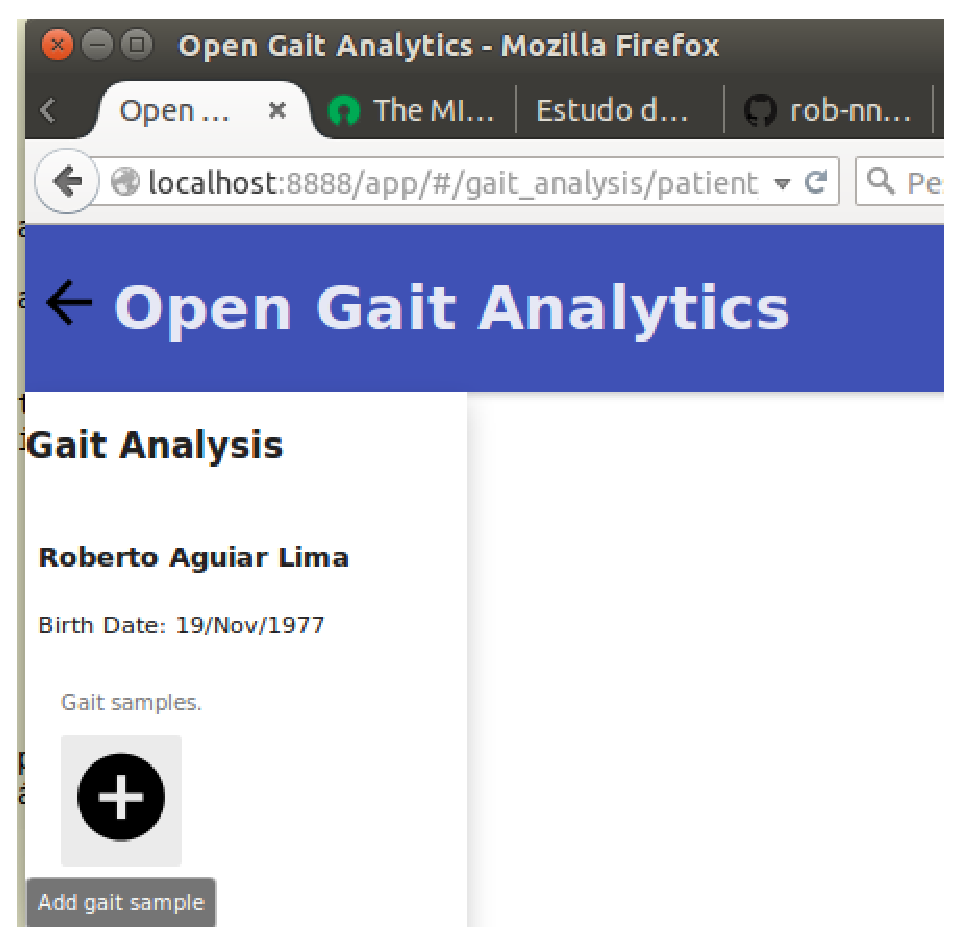
\includegraphics[width=7cm]{figuras/tela4.eps}
	\caption{Tela inicial da dados coletados do paciente.}
	\label{tela4}
\end{figure}

O usuário deve então informar a descrição da coleta e a data que a mesma ocorreu e salvar ests informações, conforme a Figura \ref{tela5}.

\begin{figure}[ht]
	\centering
	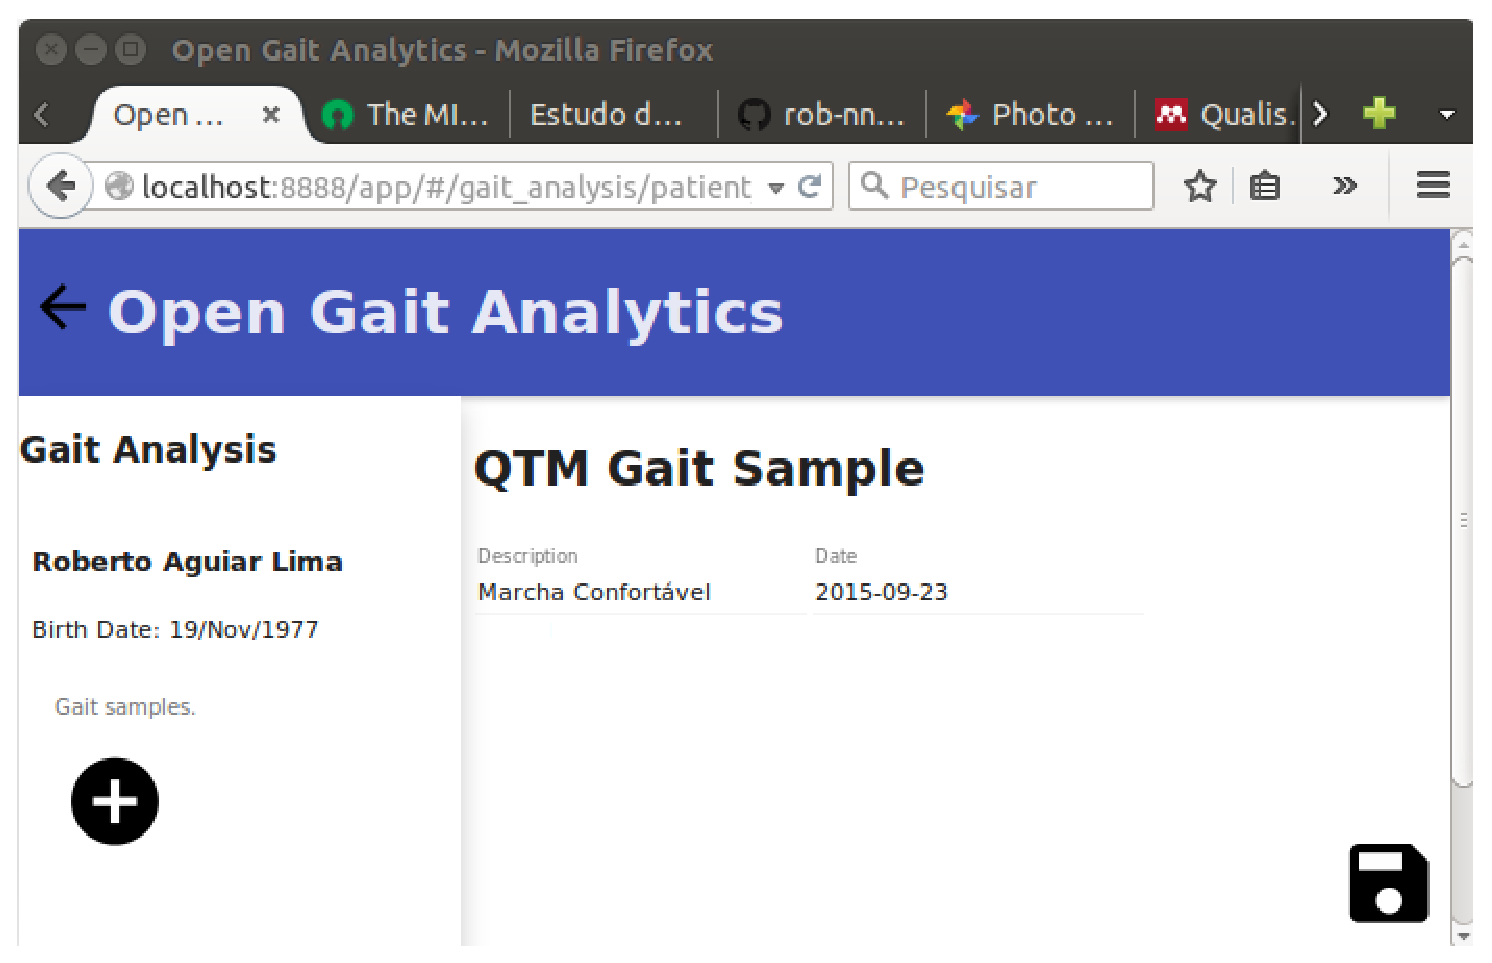
\includegraphics[width=15cm]{figuras/tela5.eps}
	\caption{Inclusão de amostra de marcha}

	\label{tela5}
\end{figure}

Depois de salva as informações o sistema pede para que o usuário selecione o arquivo proveniente do \emph{QTM}, conforme a Figura \ref{tela6}.

\begin{figure}[ht]
	\centering
	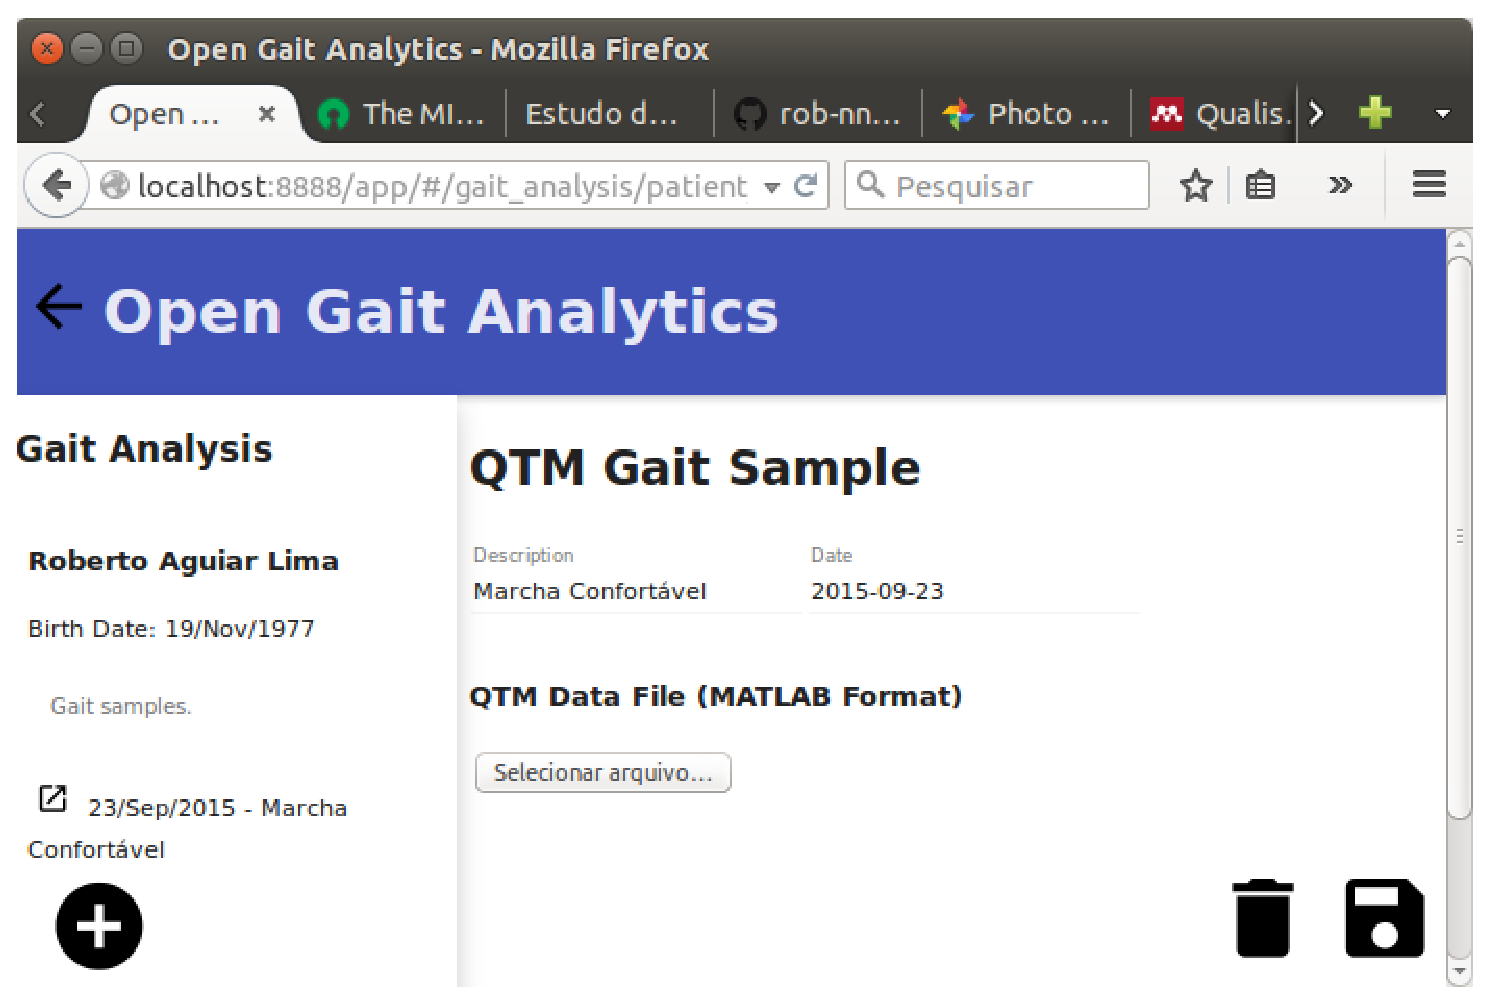
\includegraphics[width=15cm]{figuras/tela6.eps}
	\caption{Seleção do arquivo no formato \emph{MATLAB} proveniente do \emph{QTM}.}
	\label{tela6}
\end{figure}

Depois de selecionado o arquivo com os dados da marcha, seus dados são mostrados para o usuário, conforme a Figura \ref{tela7}.


\begin{figure}[ht]
	\centering
	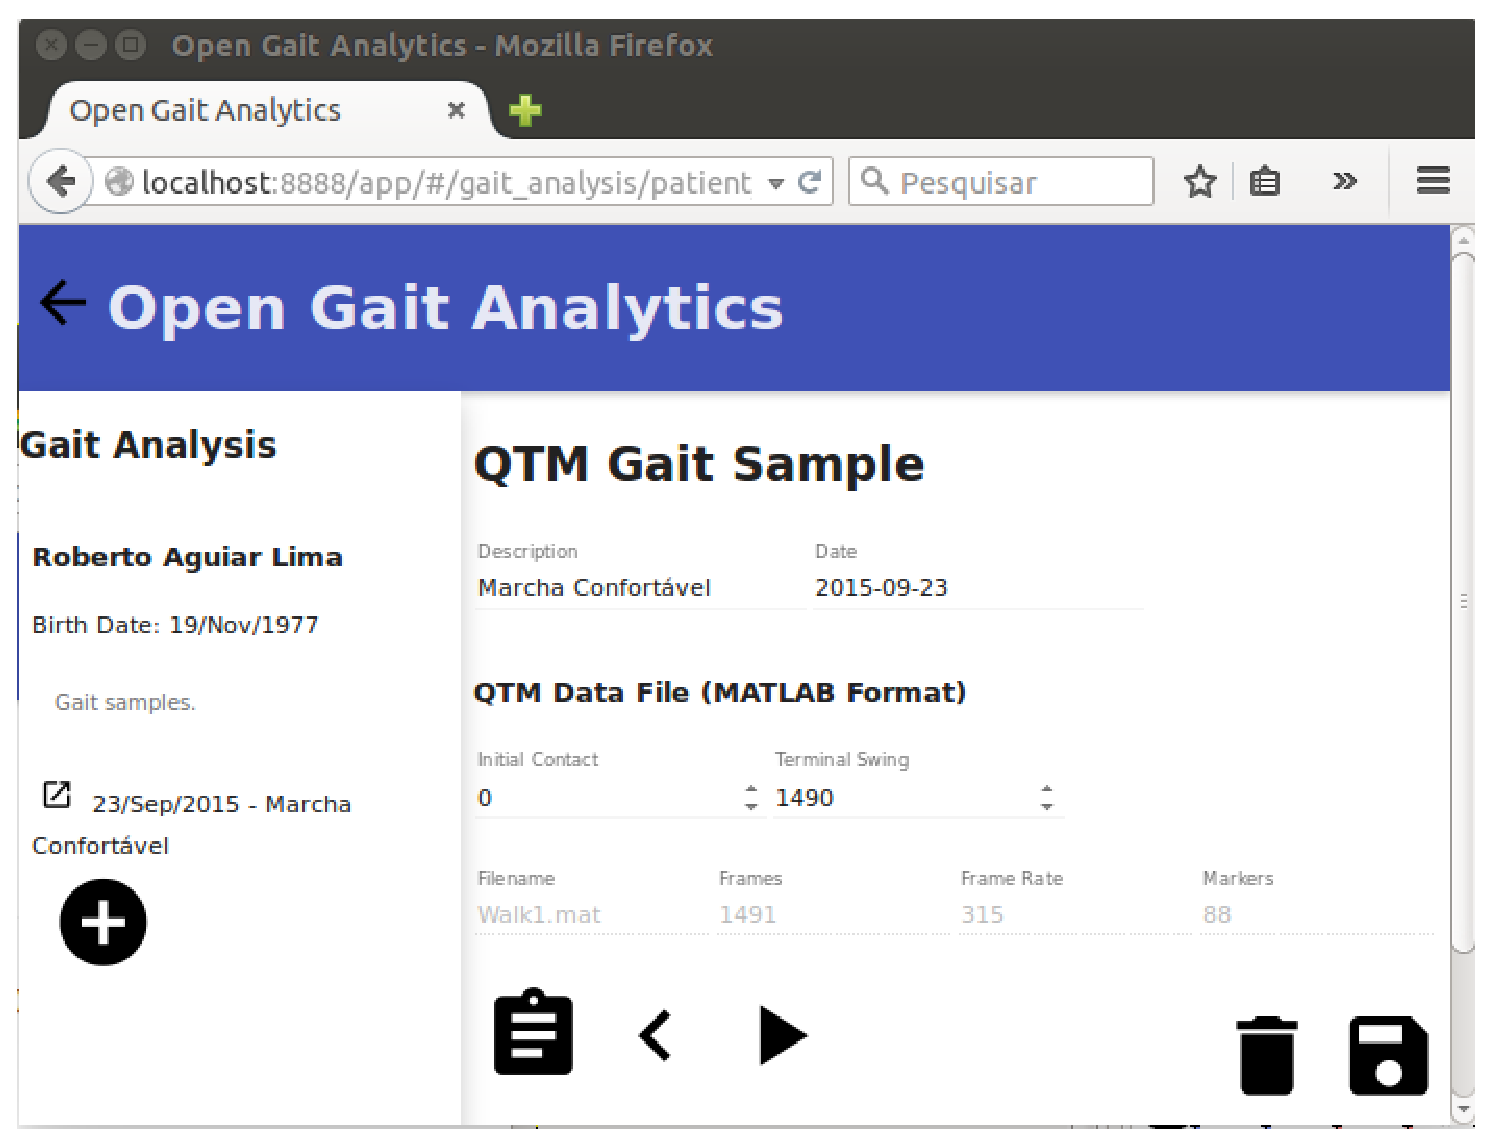
\includegraphics[width=15cm]{figuras/tela7.eps}
	\caption{Dados do arquivo provenientes do \emph{QTM}}.
	\label{tela7}
\end{figure}


Neste momento se o usuário quiser visualizar uma animação dos dados, basta clicar na seta negra que aponta para a direita que uma animação será mostra conforme a Figura \ref{animacao1}.
Esta animação foi construída usando a tecnologia \emph{ThreeJS}, resumida na seção \ref{threejs_sec}. Uma das grandes vantagens desta característica do software em relação ao \emph{QTM}, que também a possui, é o fato de que a animação está rodando num \emph{browser web} moderno, ou seja qualquer um com um \emph{browser} assim pode vê-la sem precisar do \emph{QTM} instalado. 
Além do mais como o projeto pode continuar, fica a critério dos usuários decidirem que novas características seriam interessantes, não somente nas animações, mas em todo o software.

A tela da animação também possui controle de pespectivas, ver Figura \ref{animacao2}, controle de \emph{zoom}, ver Figura \ref{animacao3}, e controle \emph{pan}, ver Figura \ref{animacao3}.
Também foram implementados, até o momento, botões de \emph{play, pause}, fechar e um contador de \emph{frames}, ver Figura \emph{animacao4a}.


\begin{figure}[ht]
  \centering
  \begin{minipage}[b]{0.32\textwidth}
    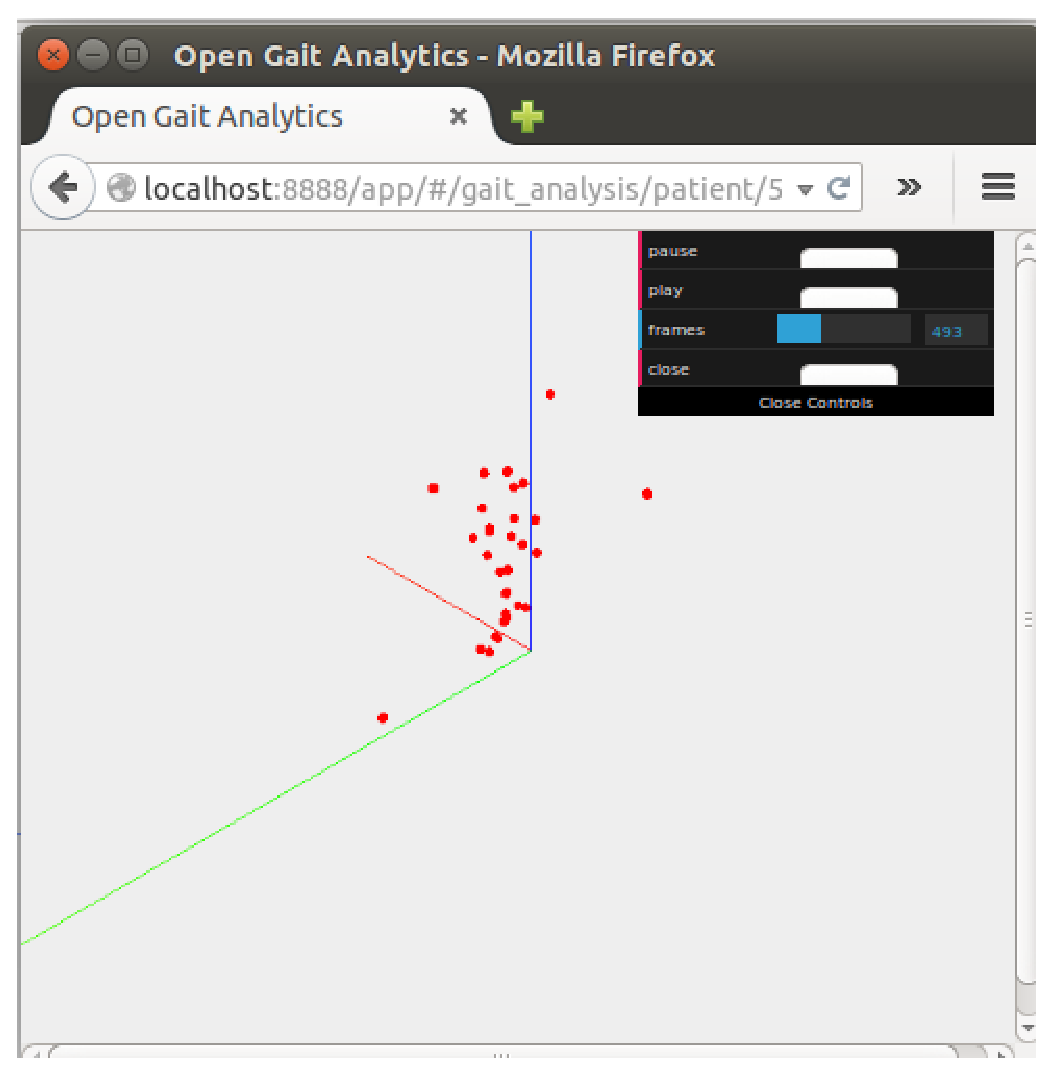
\includegraphics[width=\textwidth]{figuras/tela8.eps}
  \end{minipage}
  \hfill
  \begin{minipage}[b]{0.32\textwidth}
    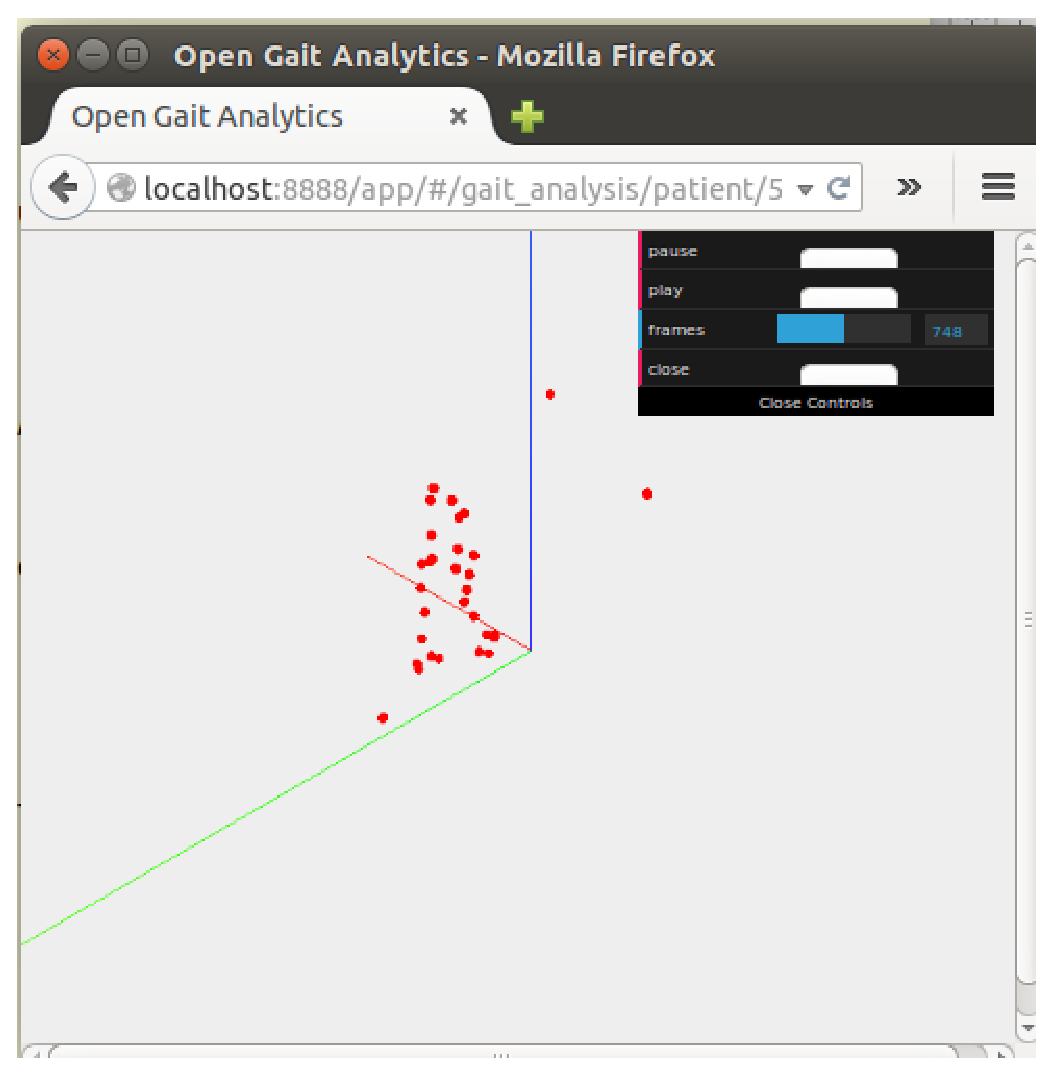
\includegraphics[width=\textwidth]{figuras/tela9.eps}
  \end{minipage}
  \hfill
  \begin{minipage}[b]{0.32\textwidth}
    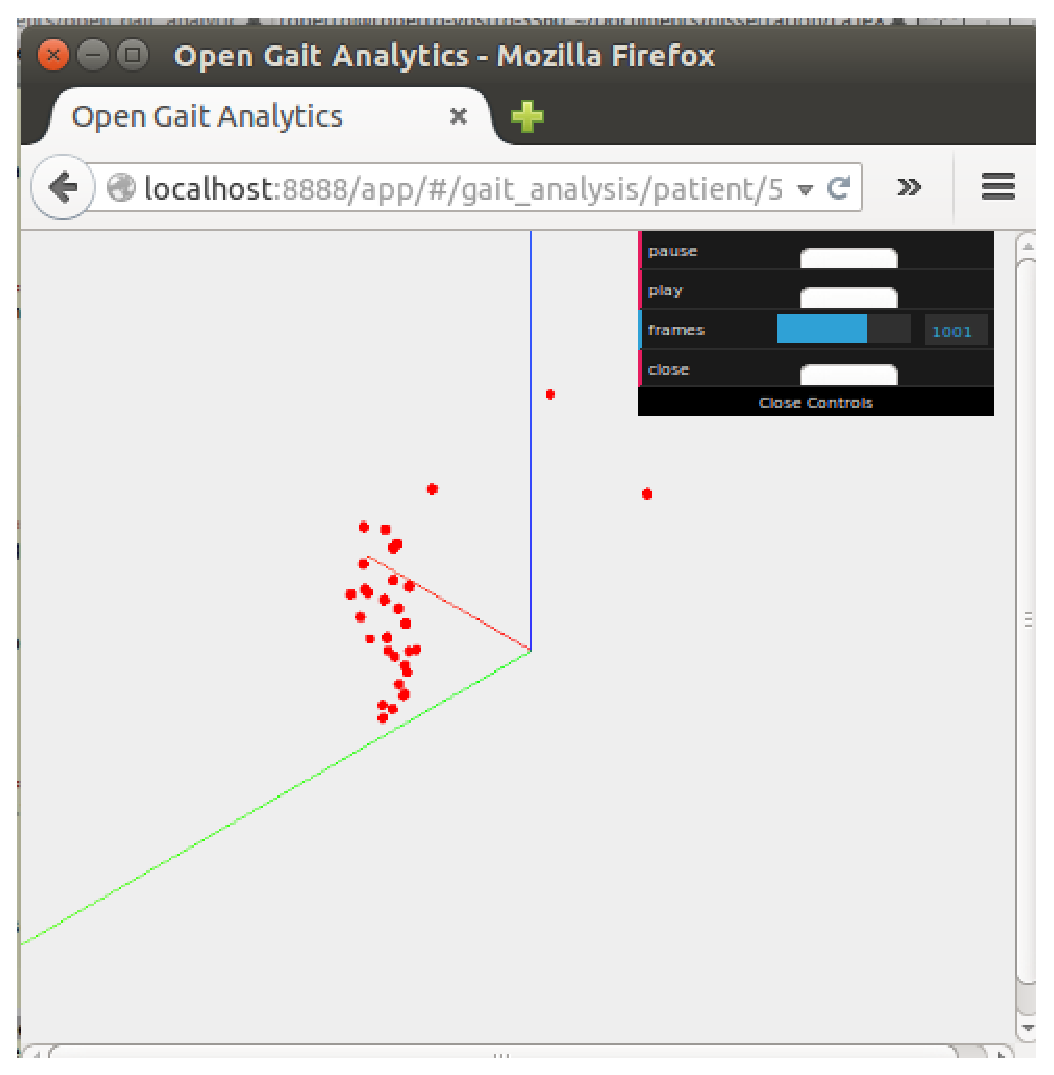
\includegraphics[width=\textwidth]{figuras/tela10.eps}
  \end{minipage}
  \caption{Animação dos marcadores em 3D.}
  \label{animacao1}
\end{figure}


\begin{figure}[ht]
  \centering
  \begin{minipage}[b]{0.49\textwidth}
    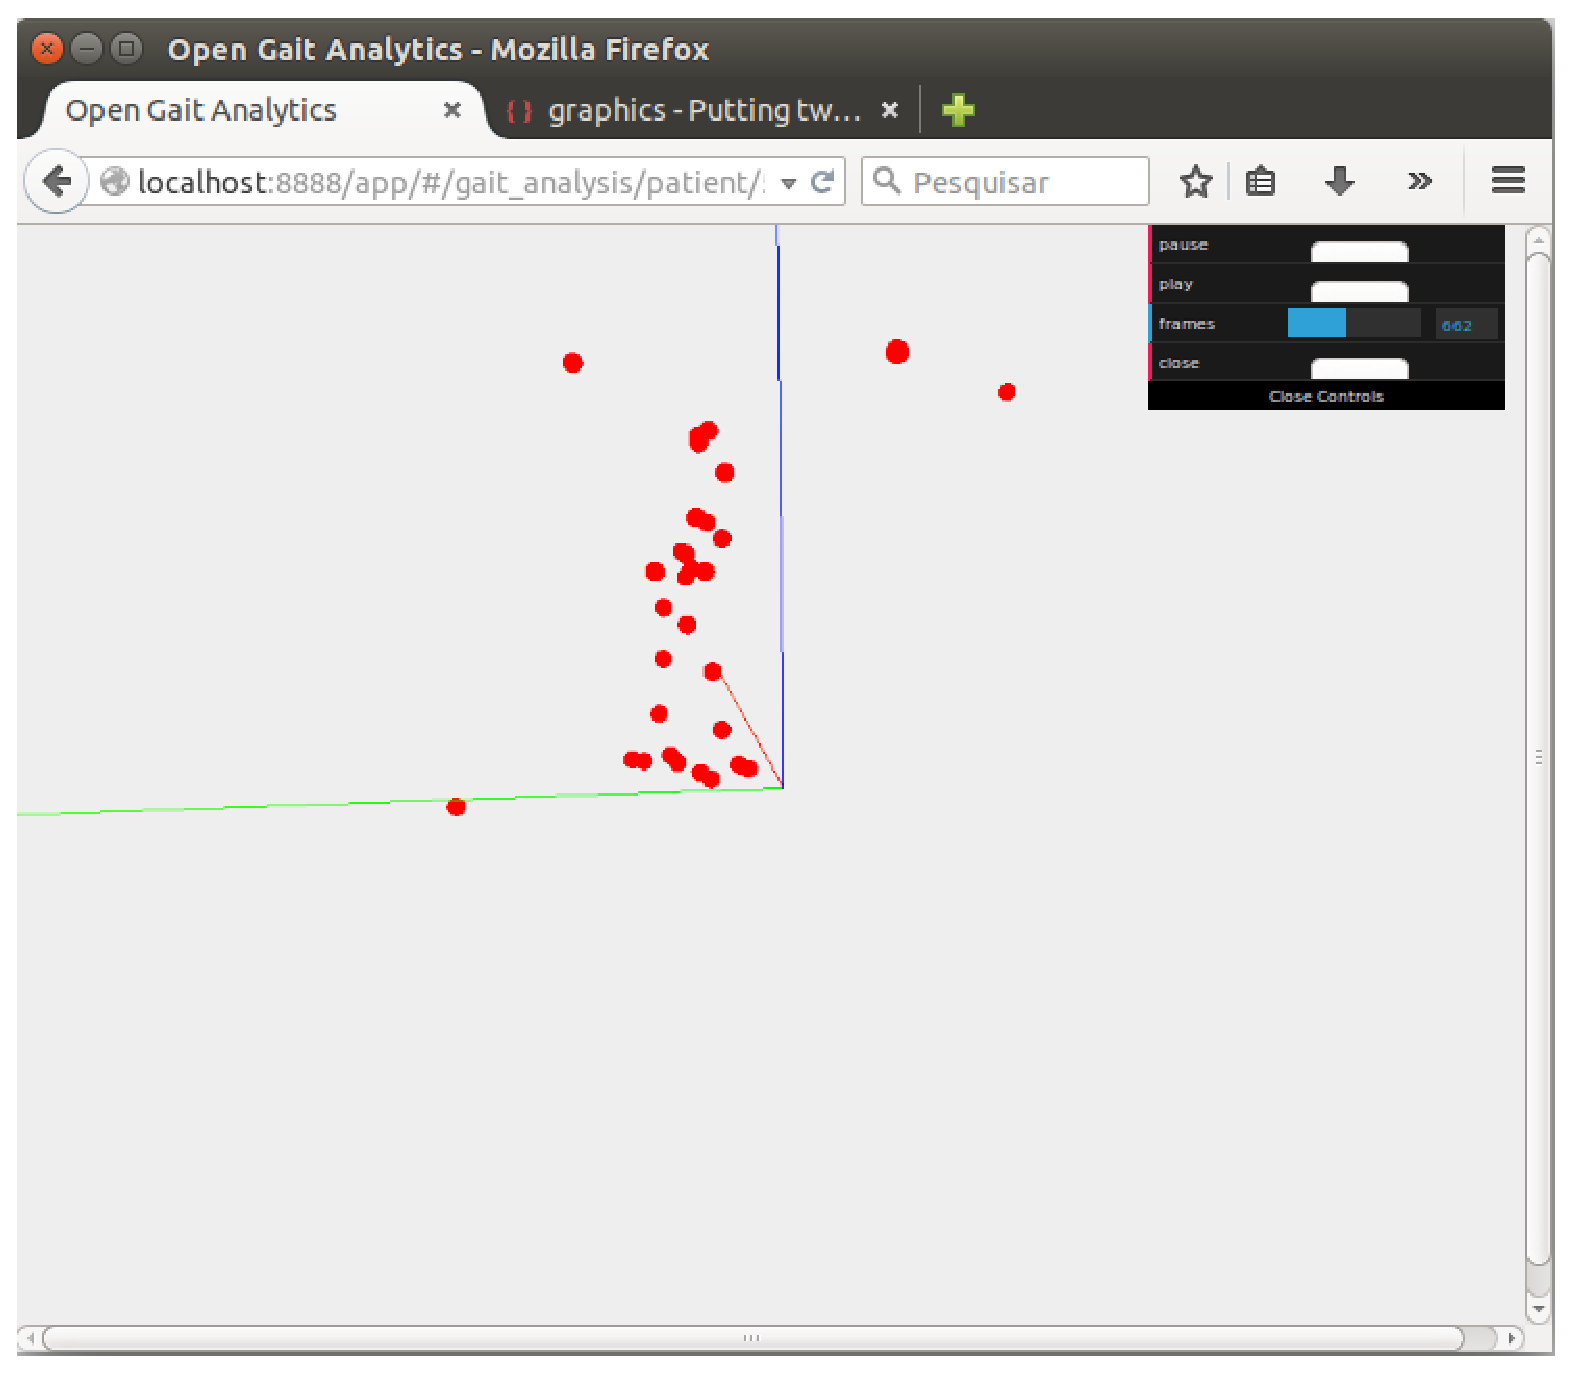
\includegraphics[width=\textwidth]{figuras/tela11.eps}
  \end{minipage}
  \hfill
  \begin{minipage}[b]{0.49\textwidth}
    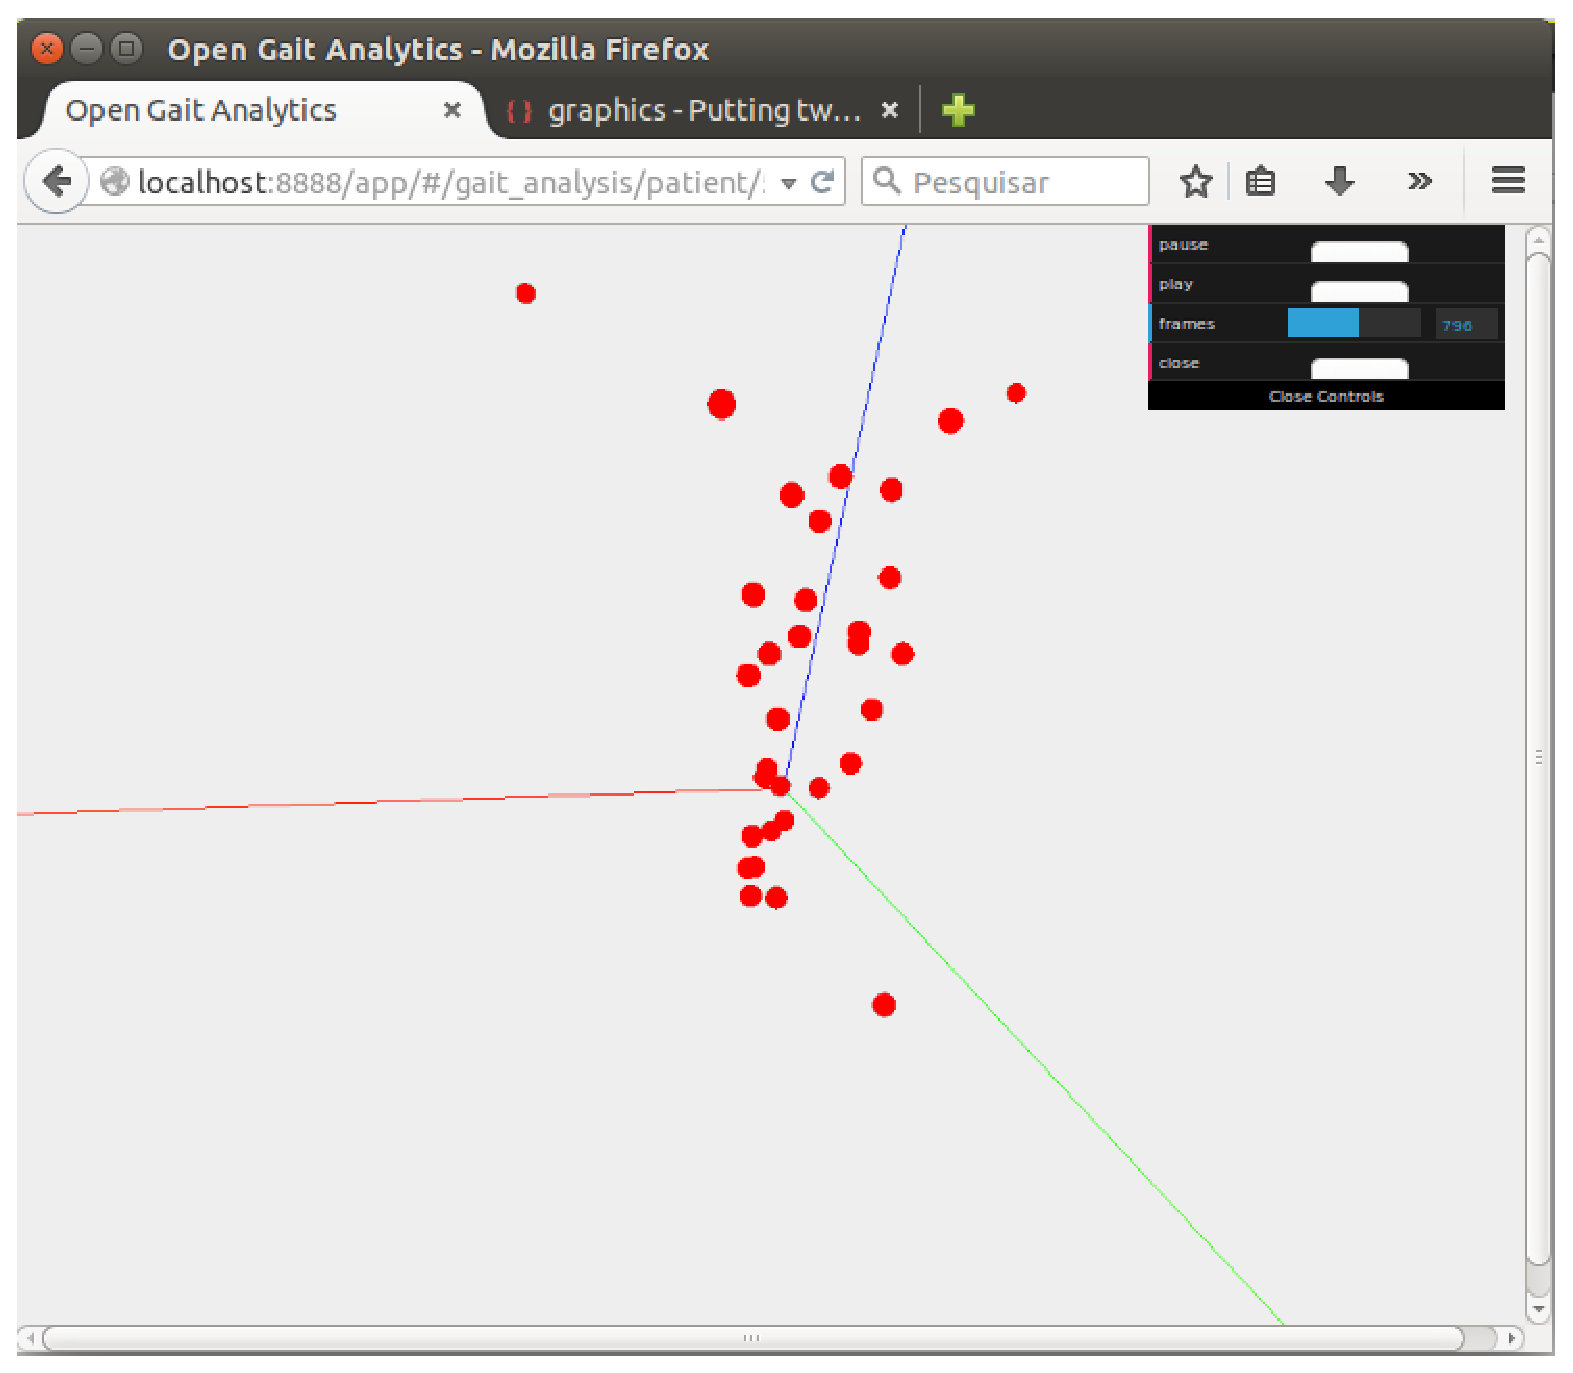
\includegraphics[width=\textwidth]{figuras/tela12.eps}
  \end{minipage}
  \caption{Controle de perspectivas.}
  \label{animacao2}
\end{figure}

\begin{figure}[ht]
  \centering
  \begin{minipage}[b]{0.49\textwidth}
    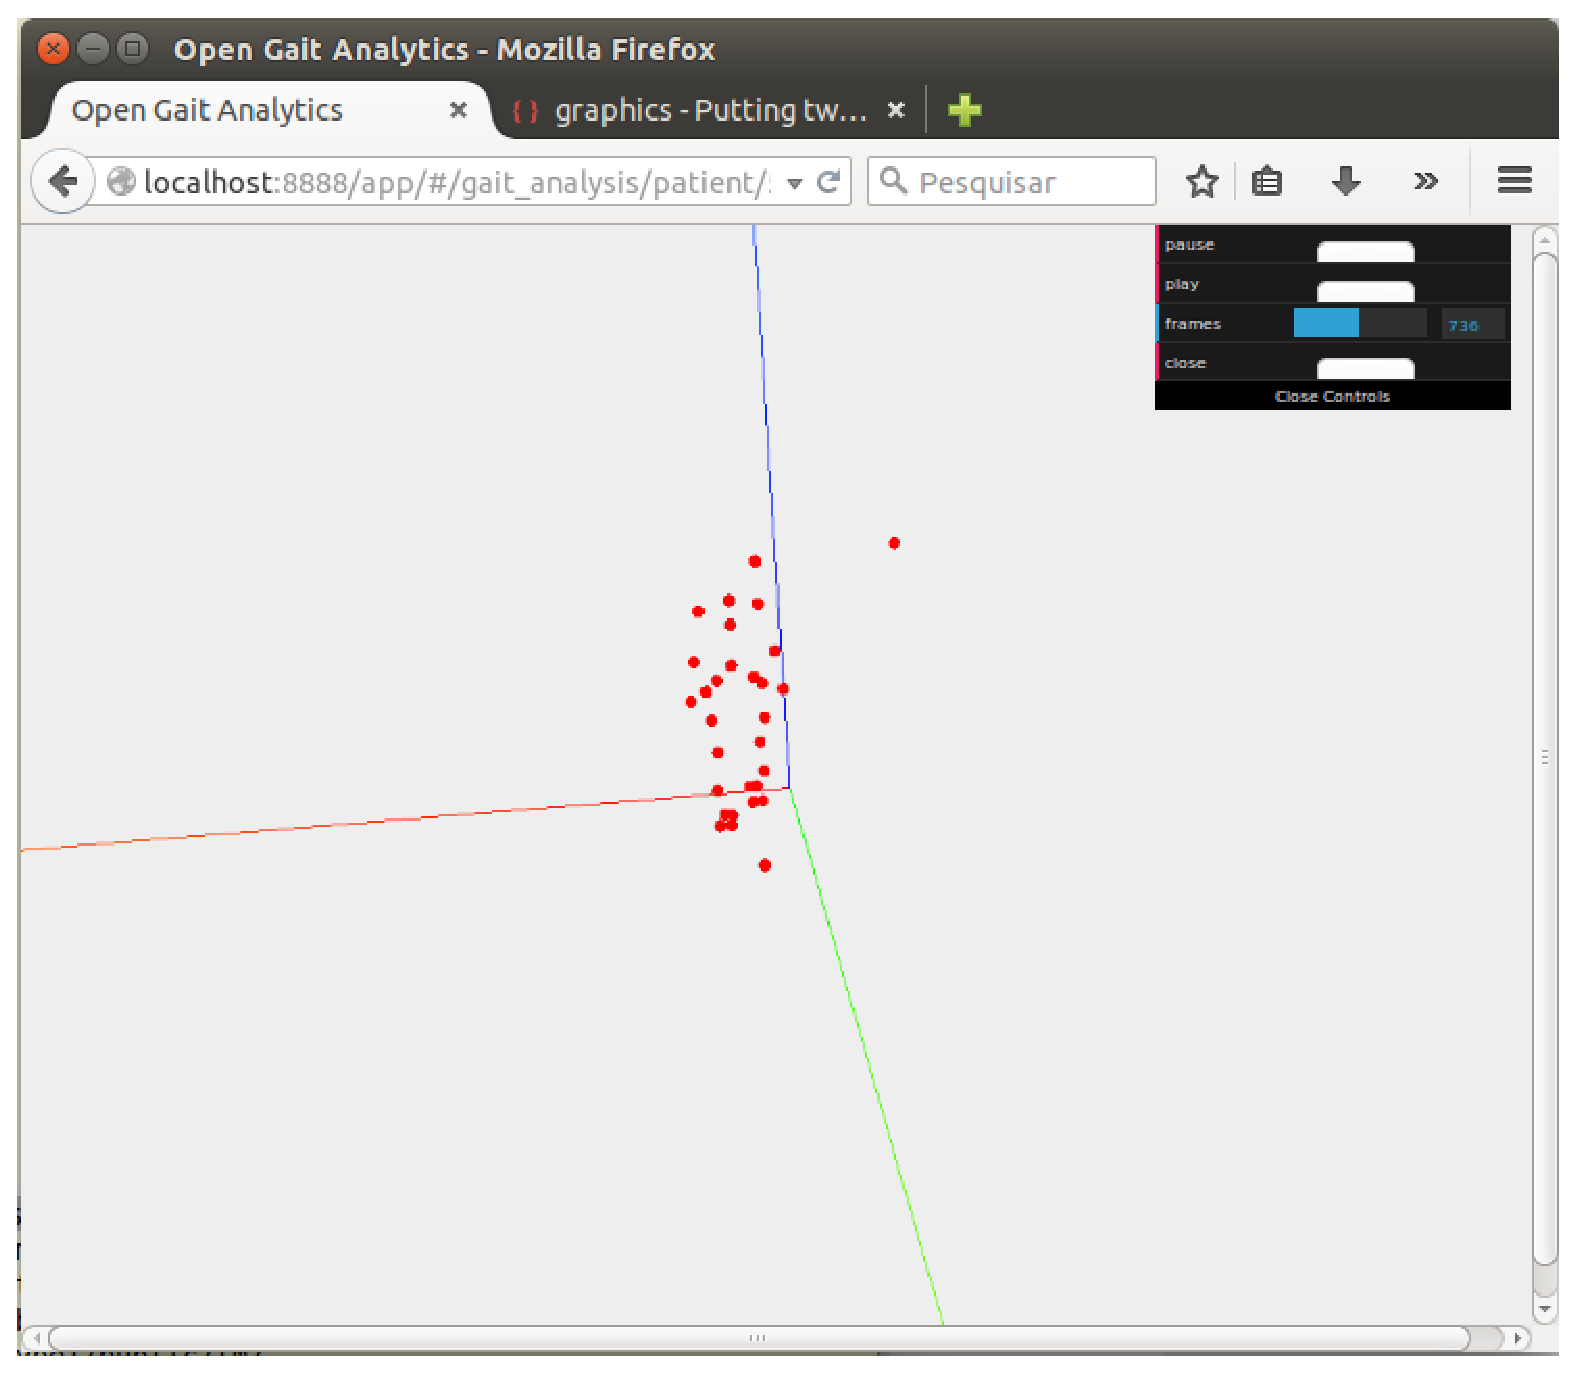
\includegraphics[width=\textwidth]{figuras/tela13.eps}
  \end{minipage}
  \hfill
  \begin{minipage}[b]{0.49\textwidth}
    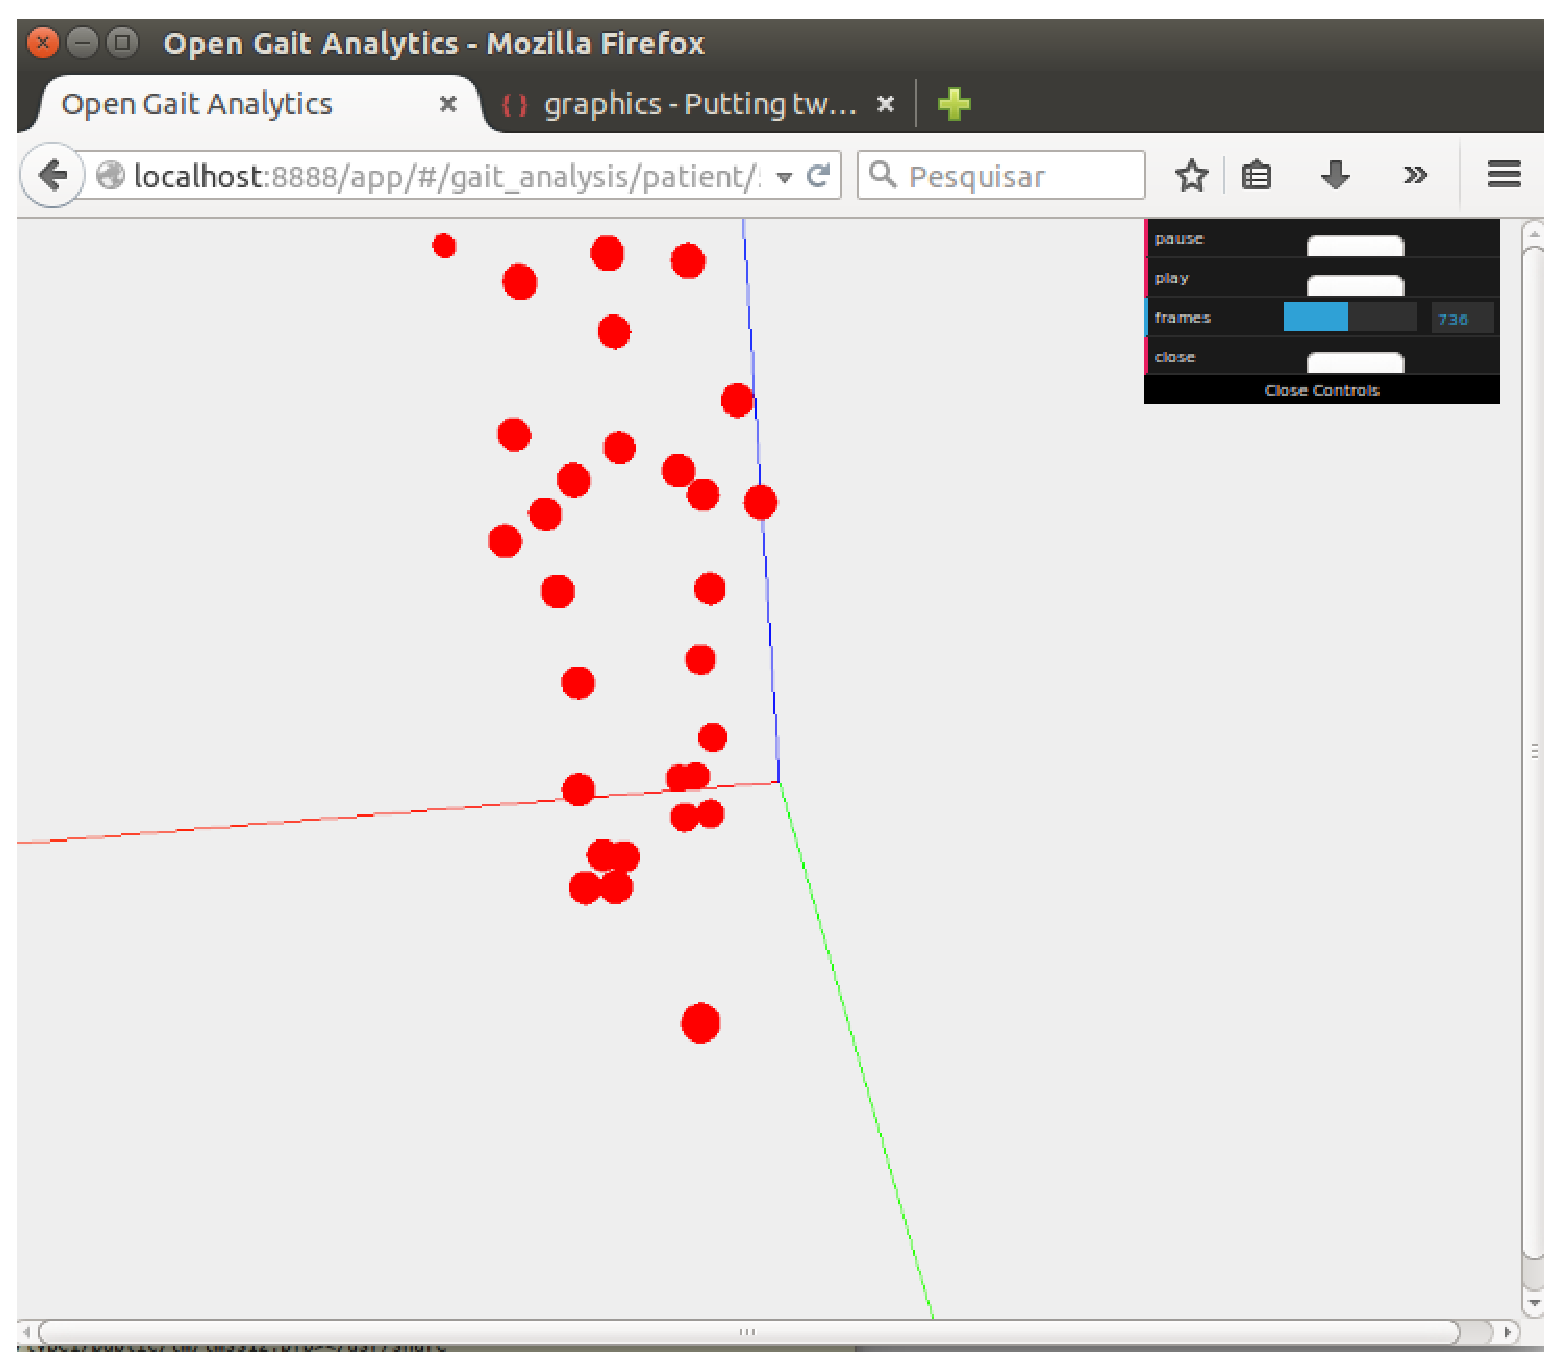
\includegraphics[width=\textwidth]{figuras/tela14.eps}
  \end{minipage}
  \caption{Controle de \emph{zoom}.}
  \label{animacao3}
\end{figure}

\begin{figure}[ht]
  \centering
  \begin{minipage}[b]{0.49\textwidth}
    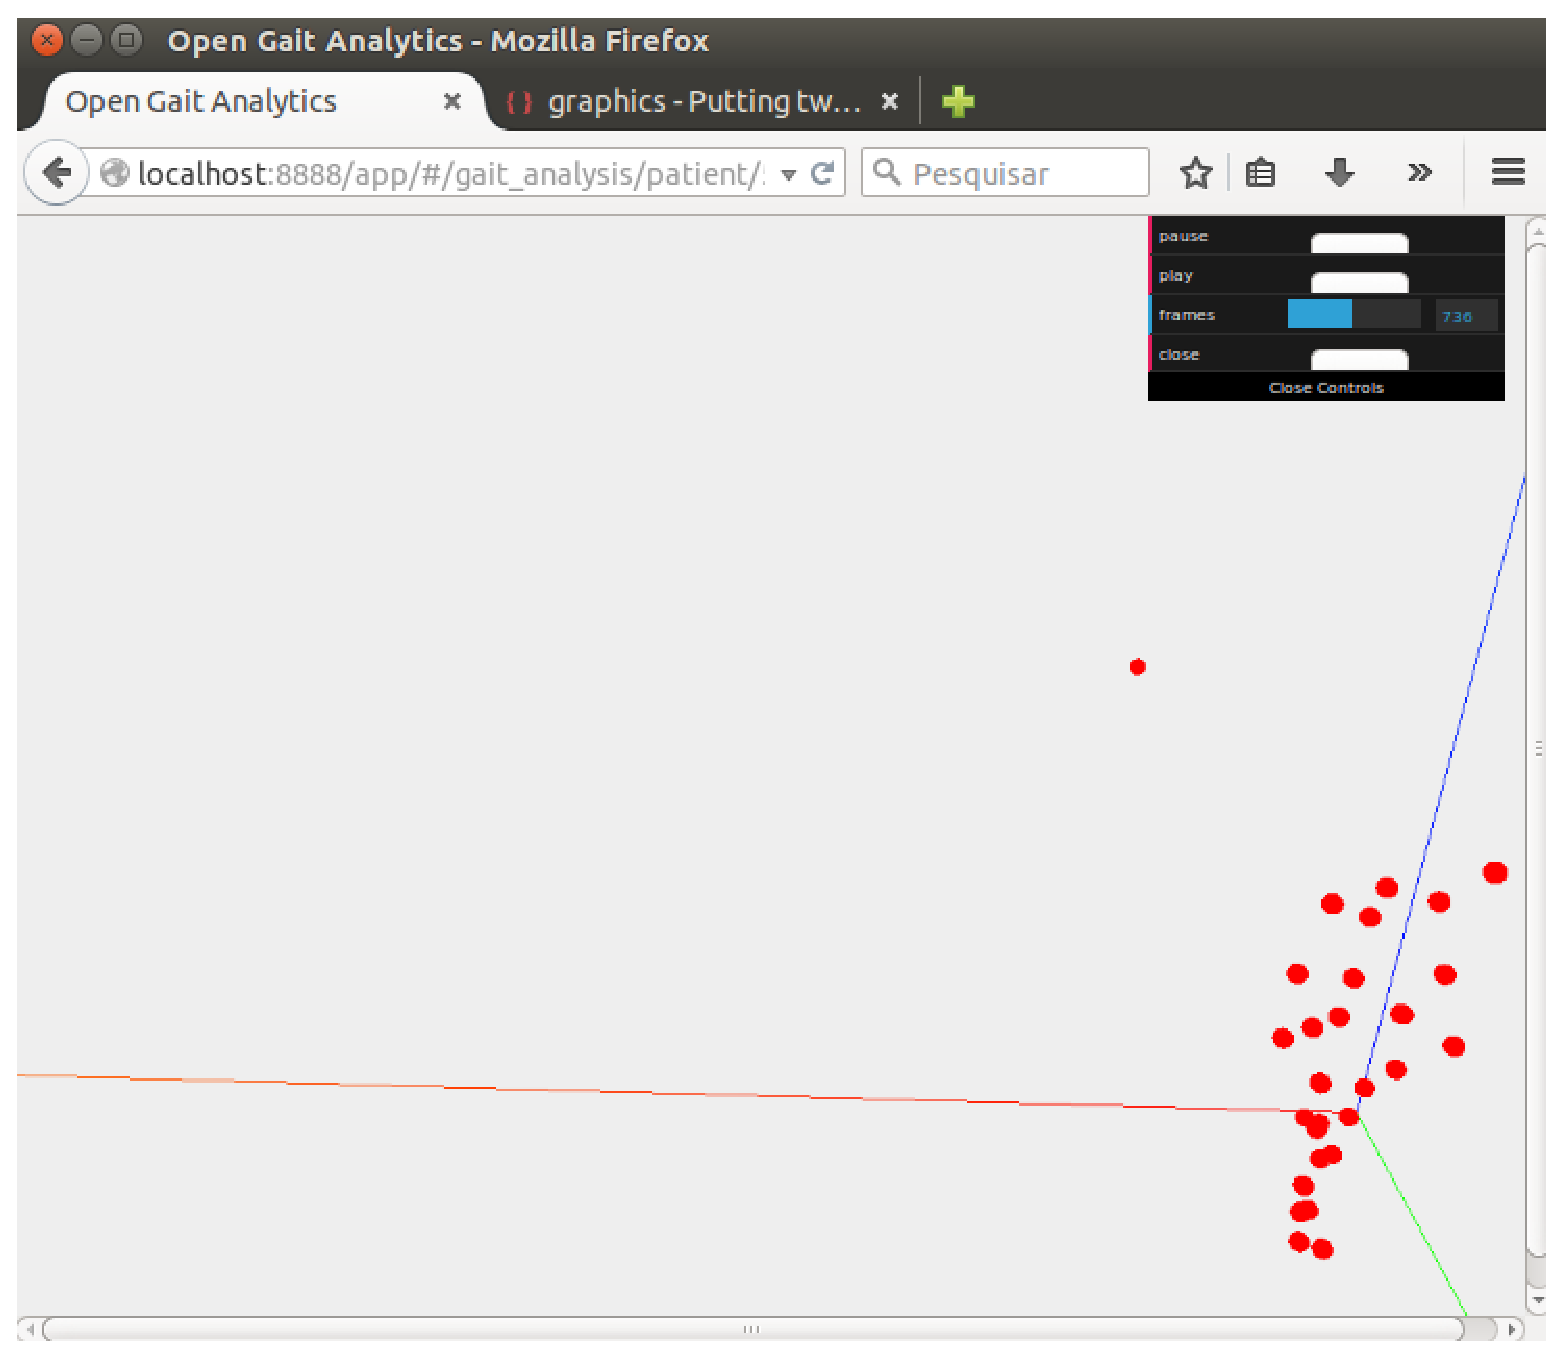
\includegraphics[width=\textwidth]{figuras/tela15.eps}
  \end{minipage}
  \hfill
  \begin{minipage}[b]{0.49\textwidth}
    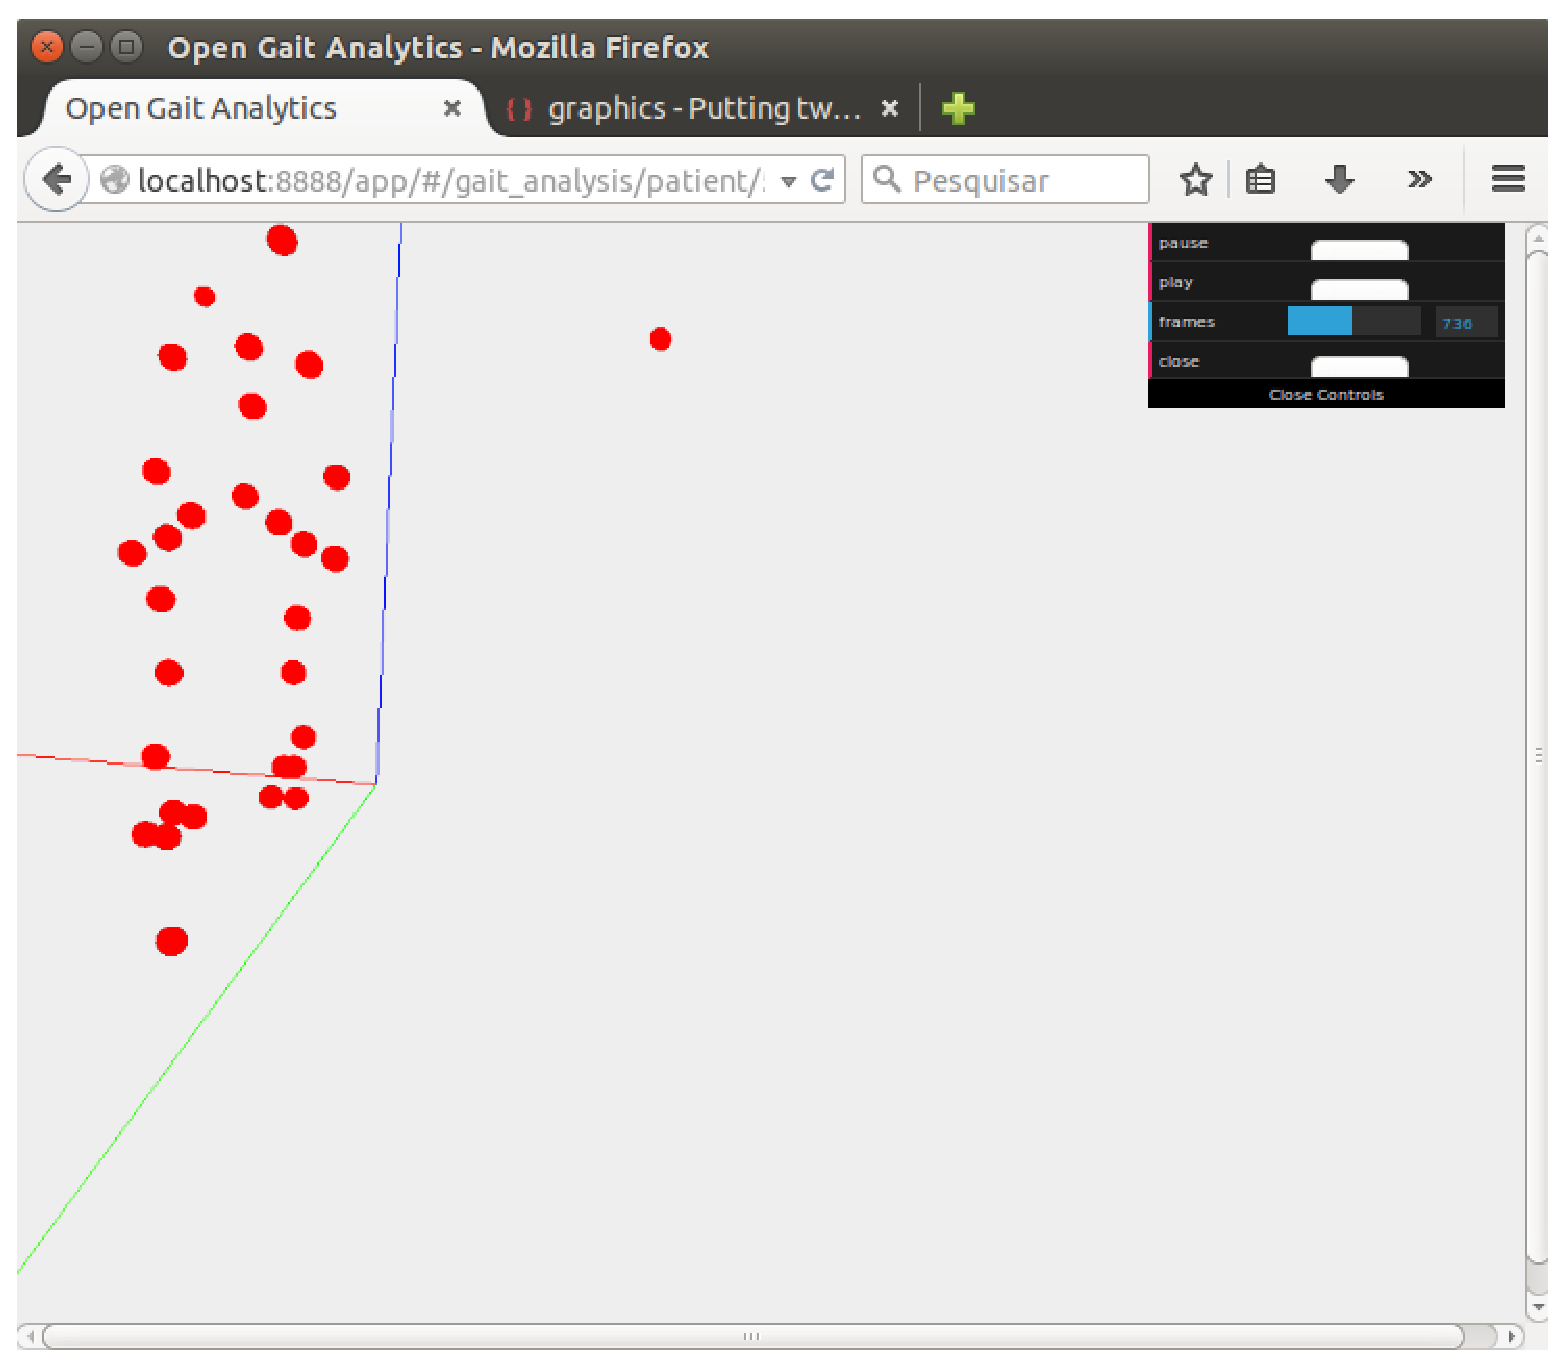
\includegraphics[width=\textwidth]{figuras/tela16.eps}
  \end{minipage}
  \caption{Controle \emph{pan}.}
  \label{animacao4}
\end{figure}

\begin{figure}[ht]
	\centering
	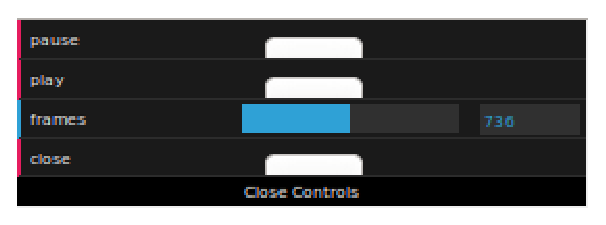
\includegraphics[width=7cm]{figuras/tela17.eps}
	\caption{Controles da animação.}
	\label{animacao5}
\end{figure}




É de fundamental importância que o usuário configure os parâmetros \emph{Initial Contact} e \emph{Terminal Swing} mostrados na Figura \ref{tela7}. Sem estes parâmetros os gráficos, vão mostrar os sinais nas fases erradas do ciclo de marcha.
A técnica que se recomenda, é inicializar a animação e quando o usuário perceber o \emph{initial contact}, pressionar o botão pause e anotar o frame. Fazer a mesma coisa para o \emph{terminal swing}.

Outra opção disponível na Figura \ref{tela7}, é a opção \emph{Markers}, esta opção permite nomear os marcadorese visualizar sua progressão espacial. A Figura \ref{tela18} mostra o resultado de se selecionar esta opção.
Ao clicar no botão ao lado de algum marcador, sua progressão no espaço é mostrada num gráfico como o da Figura \ref{tela19}. O domínio é o percentual do ciclo de marcha, já a imagem são dados espaciais brutos oriundos do \emph{QTM}.

A nomeação dos marcadores, não é uma tarefa trivial. Para isso foi criada uma ferramenta dentro da animação para ajudar com esta tarefa. Primeiro deve-se entrar na animação, depois pausá-la, e posicionar a visualização de uma forma que ajude a detectar o marcador procurado. Veja a figura \ref{tela20}, nela um marcador foi clicado com o \emph{mouse}, o marcador ficou azul e ao seu lado ele mostra o índice 30. 
Agora é só voltar na opção de marcadores, procurar o índice 30 (\emph{Marker 30}) e colocar o nome desejado. No caso deste marcador o nome é joelho esquerdo (\emph{left knee}), ver a Figura \ref{tela21}.
Agora para o sistema o marcador 30 é sempre o joelho esquerdo, veja a Figura \ref{tela22}.

\begin{figure}[ht]
	\centering
	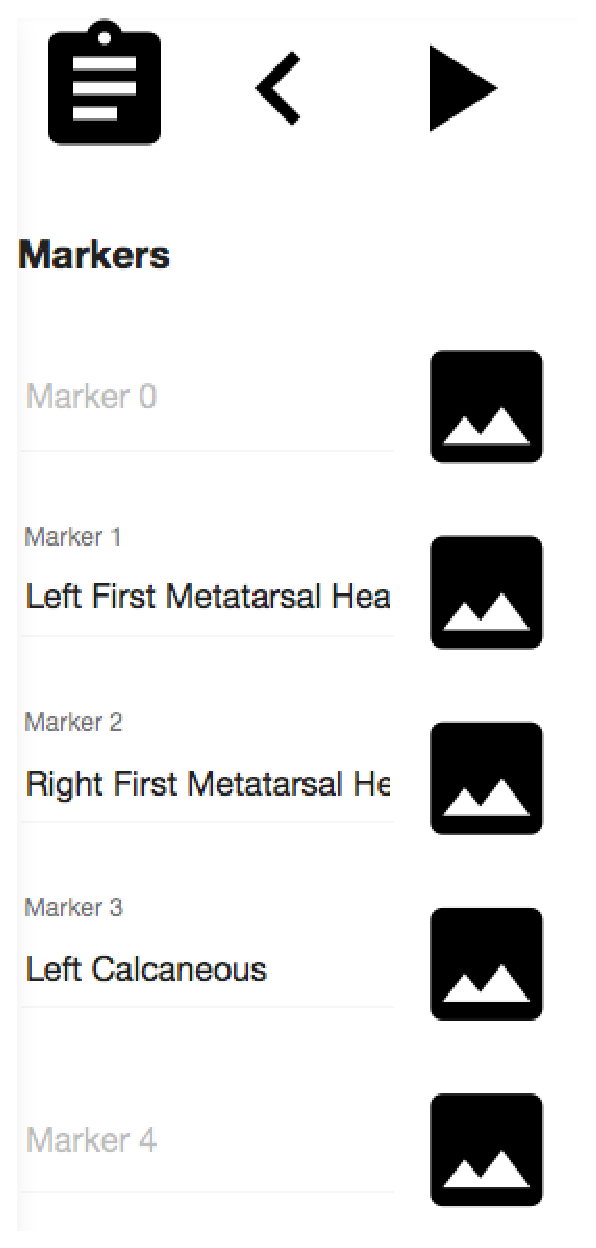
\includegraphics[width=5cm]{figuras/tela18.eps}
	\caption{Opção \emph{markers}.}
	\label{tela18}
\end{figure}


\begin{figure}[ht]
	\centering
	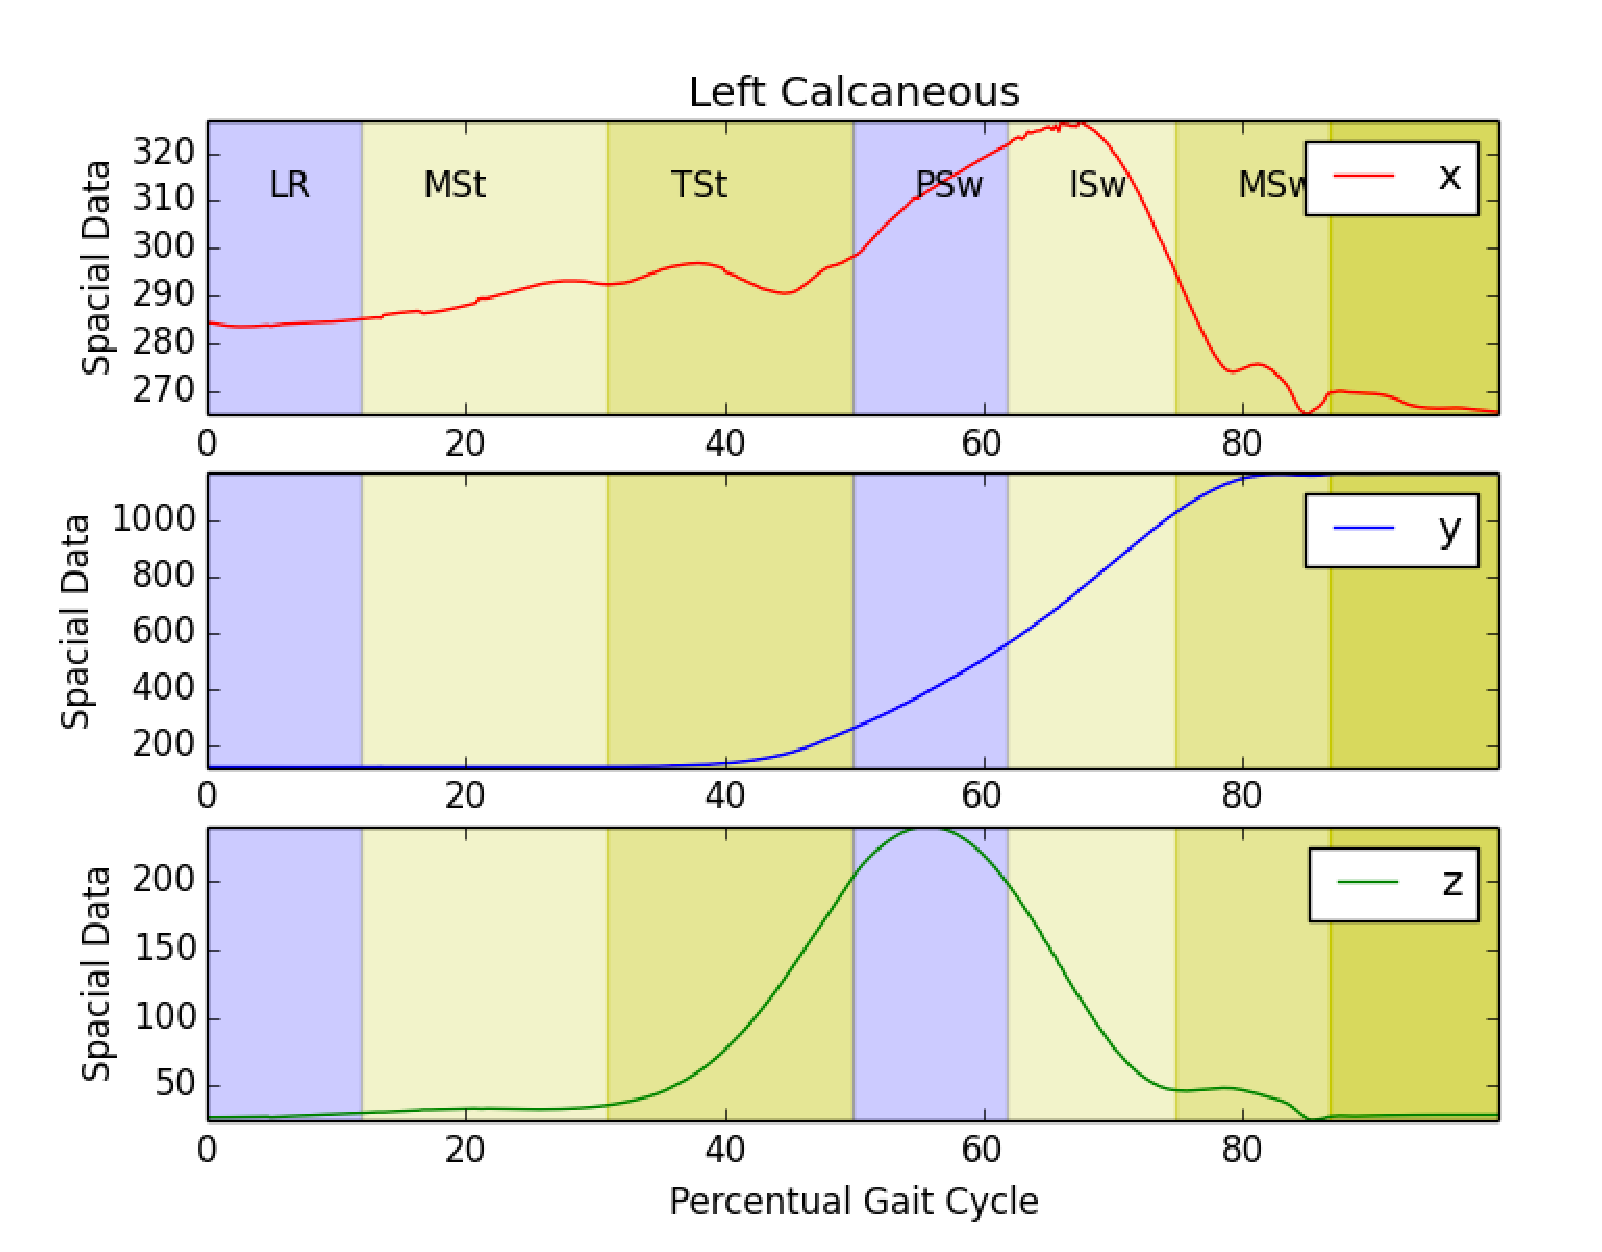
\includegraphics[width=10cm]{figuras/tela19.eps}
	\caption{Progreção espacial de um marcador.}
	\label{tela19}
\end{figure}

\begin{figure}[ht]
	\centering
	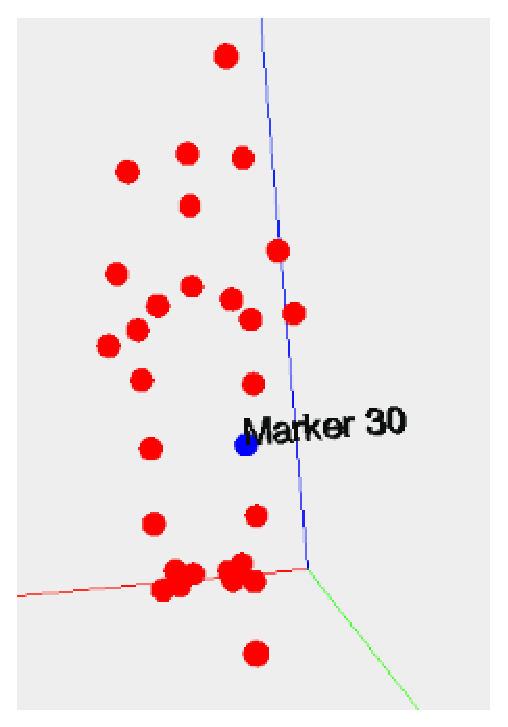
\includegraphics[width=5cm]{figuras/tela20.eps}
	\caption{Seleção de um marcador pelo \emph{mouse}.}
\label{tela20}
\end{figure}


\begin{figure}[ht]
	\centering
	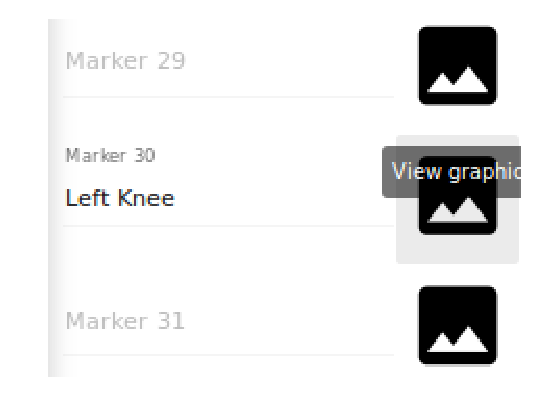
\includegraphics[width=5cm]{figuras/tela21.eps}
	\caption{Alterando o nome de um marcador}
\label{tela21}
\end{figure}

\begin{figure}[ht]
	\centering
	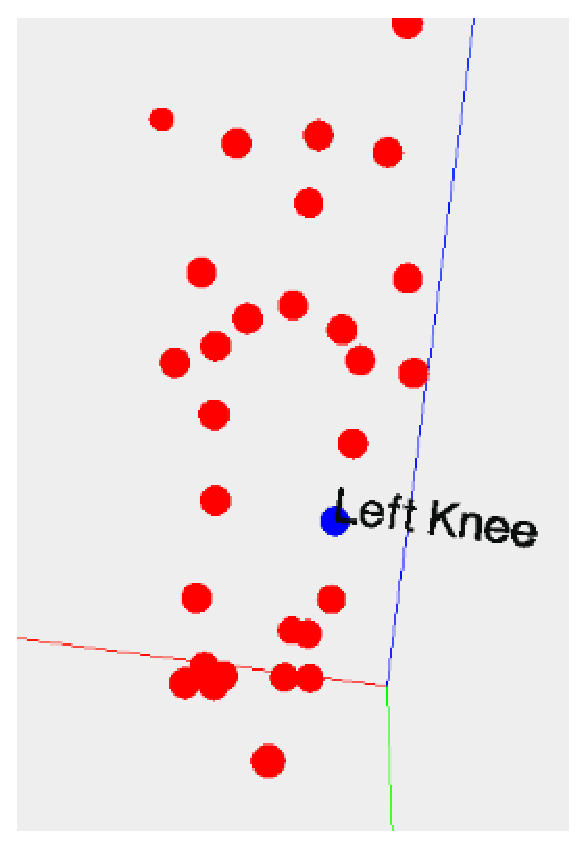
\includegraphics[width=5cm]{figuras/tela22.eps}
	\caption{Animação mostrando o marcador renomeado.}
\label{tela22}
\end{figure}

Outra funcionalidade importante é o gerador de ângulos. Esta opção está disponível da Figura \ref{tela7}. E após selecionada é mostrada na Figura \ref{tela23}.
